% ================================================================

\chapter{Resultados e discussão}
\label{cap:resultados}

Os resultados obtidos na modelagem do equilíbrio líquido-líquido dos sistemas ternários \{triglicerídeo + álcool + líquido iônico prótico\} a 298,15~K são apresentados neste capítulo segundo os dois modelos empregados, o UNIFAC-LL e o COSMO-SAC. Como não há, na literatura, dados experimentais de equilíbrio de fases para nenhum dos doze sistemas estudados (Seção~\ref{sec:dados_validacao}), não é possível verificar as predições contra medida direta nem arbitrar entre os dois modelos quando eles divergem, de modo que o que se apresenta adiante é a descrição do que cada modelo prevê, acompanhada da procedência e das incertezas de cada dado de entrada.

A exposição parte da validação da ferramenta computacional (Seção~\ref{sec:validacao_computacional}), passa à descrição do comportamento de fases previsto por cada modelo (Seção~\ref{sec:resultados_por_sistema}), confronta esses resultados com a hipótese de cossolvência que motiva o trabalho (Seção~\ref{sec:cossolvencia}), discute os mecanismos moleculares que sustentariam o comportamento observado (Seção~\ref{sec:interpretacao_fisicoquimica}) e encerra com a síntese do que os dois modelos estabelecem em conjunto, daquilo em que divergem e do que permanece indeterminado (Seção~\ref{subsec:sintese}).

\section{Validação da ferramenta computacional}
\label{sec:validacao_computacional}

Os resultados discutidos ao longo deste capítulo dependem inteiramente da correção da ferramenta computacional empregada para gerar os diagramas de equilíbrio líquido-líquido, e essa correção foi estabelecida em duas etapas complementares. A primeira isola o motor de cálculo, isto é, os algoritmos de estabilidade de fases, flash líquido-líquido e localização do ponto crítico, testando-o independentemente do modelo termodinâmico empregado (Seção~\ref{subsec:motor_termodinamico}); a segunda caracteriza os dados de entrada específicos de cada modelo, os pares de interação do UNIFAC-LL e os perfis sigma do COSMO-SAC, incluindo o diagnóstico de qualidade que revelou o enovelamento discutido na Seção~\ref{subsec:parametros_perfis}. Tal separação entre motor e modelo é o que permite, adiante, atribuir a origem de eventuais resultados fisicamente implausíveis, distinguindo uma falha na implementação numérica de um problema na parametrização do sistema.

\subsection{Motor termodinâmico}
\label{subsec:motor_termodinamico}

Um erro na predição de um sistema ternário pode ter duas origens bastante distintas, uma falha no modelo de coeficiente de atividade (parâmetros de interação incorretos ou mal extrapolados) ou uma falha no algoritmo que consome esses coeficientes para construir o diagrama de fases, e sem isolar essas duas fontes um resultado implausível não permite saber se o problema está na termodinâmica do sistema ou na implementação. Validou-se, por esse motivo, o motor de cálculo de forma independente do modelo, empregando-se a equação de Margules simétrica de dois parâmetros ($G^E/RT = A\,x_1 x_2$, com $A = A_{12} = A_{21}$) como caso de referência para um sistema binário, por possuir solução analítica conhecida para a curva binodal. Para $A > 2$ (limiar crítico do modelo simétrico), as composições de equilíbrio $x^{I}$ e $x^{II}$ satisfazem a condição de coexistência
\[
\ln\!\left(\frac{x}{1-x}\right) + A(1-2x) = 0,
\]
resolvida analiticamente por busca de raiz unidimensional de alta precisão. Adotando-se $A = 2{,}5$, a solução exata fornece $x^{I} = (0{,}1448,\ 0{,}8552)$ e $x^{II} = (0{,}8552,\ 0{,}1448)$, e o mesmo sistema, resolvido pelo motor completo (teste de estabilidade por TPD seguido de flash por Rachford-Rice com substituições sucessivas), convergiu para os mesmos valores, com desvio quadrático médio de $2{,}50 \times 10^{-7}$ em relação à solução analítica, o que confirma a corretude da implementação independentemente do modelo termodinâmico empregado.

O teste de estabilidade de fases foi implementado segundo o critério do plano tangente (\textit{tangent plane distance}, TPD), na formulação de Baker, Pierce e Luks e posteriormente sistematizada por Michelsen, que verifica se uma composição testada minimiza a energia livre de Gibbs da mistura em relação a qualquer perturbação de composição, sendo a composição instável, e o sistema separado em duas fases líquidas, sempre que essa condição não é satisfeita. O cálculo de flash líquido-líquido, por sua vez, foi resolvido pelo método de Rachford-Rice com substituições sucessivas, adotando-se como critérios de aceitação da solução não trivial $0{,}01 < \psi < 0{,}99$ e $|x^{\alpha} - x^{\beta}| > 0{,}02$, de modo a descartar convergências para a solução trivial (as duas fases coincidindo), problema numérico recorrente nesse tipo de algoritmo quando a estimativa inicial é inadequada. Já o ponto crítico da binodal, onde as duas fases líquidas tornam-se indistinguíveis, foi localizado por encolhimento sucessivo da largura da região instável, procedimento que se mostrou numericamente mais estável do que a alternativa inicialmente testada, baseada em Newton-Raphson aplicado à condição de forma cúbica da superfície de Gibbs.

\subsection{Parâmetros e perfis de entrada}
\label{subsec:parametros_perfis}

Validado o motor de cálculo, resta caracterizar os dados que o alimentam em cada um dos dois casos, uma vez que o UNIFAC-LL e o COSMO-SAC consomem informações de naturezas distintas (parâmetros de interação entre pares de grupos funcionais, no primeiro caso, e perfis de densidade de carga superficial, no segundo) e a procedência de cada uma precisa ser descrita separadamente. Não se pretende, aqui, estabelecer qual dos dois conjuntos de entrada é preferível, questão que os resultados deste trabalho não permitem decidir na ausência de dados experimentais de referência, mas documentar de onde veio cada dado, quais verificações se realizaram sobre ele e quais incertezas permanecem associadas a cada predição apresentada adiante.

Empregou-se, no UNIFAC-LL, a matriz de parâmetros de interação de \citeonline{magnussen1981}, que fornece a maior parte das entradas requeridas pelos sistemas estudados. Dezesseis entradas, contudo, não constam dessa tabela original (oito pares de grupos, considerados nas duas direções, uma vez que $a_{mn} \neq a_{nm}$), sendo quatro delas relativas aos grupos amino e carboxilato que compõem os líquidos iônicos próticos, nas combinações CCOO/CNH$_2$ e CNH$_2$/COO, que entram no cálculo dos doze sistemas ternários centrais deste trabalho, e as doze restantes relativas ao grupo carboxila (COOH), requeridas apenas nos sistemas com ácido graxo livre discutidos na Seção~\ref{subsec:casos_sem_separacao}. Para todas elas, adotaram-se os valores preditos pelo UNIFAC 2.0 de \citeonline{hayer2025}, reunidos na Tabela~\ref{tab:parametros_ml_pil} do Capítulo~\ref{cap:metodologia}.

Optou-se por esse preenchimento, em detrimento de uma calibração dedicada, em razão da própria escassez de dados para os grupos em questão, visto que os conjuntos experimentais disponíveis para pares que envolvam grupos amino e carboxilato em contato com ésteres de cadeia longa são pequenos e estruturalmente distantes dos sistemas-alvo, condição na qual uma regressão dedicada tende a ajustar-se às particularidades do conjunto de calibração sem garantia de generalização. Considerando-se, ainda, que o UNIFAC 2.0 preserva o arcabouço original de \citeonline{fredenslund1975} e os mesmos parâmetros $R_k$ e $Q_k$ de \citeonline{magnussen1981} para os grupos relevantes a este trabalho, a compatibilidade com o restante da matriz é direta, pois não se faz necessária qualquer conversão de escala ou termo adicional de dependência de temperatura além da forma clássica $\Psi_{mn} = \exp(-a_{mn}/T)$.

O procedimento pelo qual esses valores são obtidos condiciona a leitura dos resultados que dele dependem, e merece descrição. O UNIFAC 2.0 é um modelo de aprendizado de máquina que emprega a técnica de completamento de matriz (\textit{matrix completion}), na qual a matriz incompleta de parâmetros de interação é tratada como um objeto de baixa dimensionalidade e as entradas faltantes são inferidas a partir da estrutura estatística das entradas conhecidas, com todos os parâmetros ajustados simultaneamente contra mais de 224.000 pontos experimentais do \textit{Dortmund Data Bank} \cite{hayer2025}. Como nenhuma medida experimental nova dos pares ausentes é introduzida nesse processo, o valor adotado para um par como CCOO/CNH$_2$ ancora-se em uma inferência a partir do comportamento de outros pares presentes na base, sem que exista, por trás dele, dado de equilíbrio de fases de sistema que contenha simultaneamente esses dois grupos. Tal característica não compromete, por si só, a plausibilidade dos valores (cuja ordem de grandeza, entre dezenas e poucas centenas de Kelvin, é compatível com a dos demais parâmetros da matriz), embora delimite o alcance da predição, já que os sistemas deste trabalho combinam triglicerídeos C57 a cátions amônio protonados, combinação para a qual não se identificou sistema experimental correspondente na base de treinamento.

Durante a construção dessa matriz, observou-se ainda uma sensibilidade que merece registro. O par CCOO/COO, adotado neste trabalho com o valor de 560,20~K, participa do cálculo de todos os doze sistemas, visto que conecta o grupo éster presente nos três triglicerídeos ao grupo carboxilato do ânion hexanoato, comum aos dois líquidos iônicos próticos. Ao substituir-se esse valor por $-122{,}3$~K (registrado na base \texttt{binary.csv} distribuída com o JCOSMO), eliminou-se por completo a formação de curva binodal em todos os sistemas avaliados, inclusive naqueles em que a separação de fases aparece de forma consistente nos dois modelos. Não foi possível, dentro do escopo deste trabalho, determinar qual dos dois valores é fisicamente mais adequado, nem mapear as implicações de adotar cada um deles sobre o restante da matriz, de modo que se manteve o valor original por coerência com a parametrização de \citeonline{magnussen1981}, e a questão permanece em aberto.

Submeteu-se a implementação do UNIFAC-LL, tomada em conjunto com a matriz assim construída, a uma verificação externa contra o sistema ternário \{n-hexano + etanol + água\} a 298,15~K, escolhido por dispor de dados experimentais consolidados \cite{sorensen1980} e por ter todos os parâmetros necessários já presentes na tabela de \citeonline{magnussen1981}, o que isola a verificação da implementação da questão do preenchimento discutida acima. O desvio quadrático médio (RMSD) das frações molares nas linhas de amarração foi de 0,0872, valor compatível com a magnitude de desvio usualmente associada ao UNIFAC-LL em sistemas contendo água, o que sugere que o desvio observado reflete limitações conhecidas do modelo para esse tipo de par binário.

Do lado do COSMO-SAC, o dado de entrada é de outra natureza, pois em vez de parâmetros ajustados a pares de grupos o modelo parte do perfil sigma de cada espécie (uma distribuição da densidade de carga superficial obtida a partir da geometria molecular otimizada por cálculo quântico), que dispensa ajuste prévio a dados de equilíbrio de fases. Obtiveram-se os perfis do etanol, do metanol, da trioleína, da trilinoleína e da trilinolenina diretamente do banco de dados interno do JCOSMO, gerado a partir de cálculos GAMESS previamente validados pelo desenvolvedor da ferramenta \cite{ferrarini2018}, ao passo que os dois líquidos iônicos próticos, por não constarem desse banco, tiveram seus perfis calculados como par iônico neutro, conforme descrito na Seção~\ref{sec:dft_cosmo}. Adotou-se a parametrização COSMO-SAC-HB2 de \citeonline{hsieh2010}, que subdivide a superfície de ligação de hidrogênio em grupos do tipo hidroxila e outros grupos doadores ou aceptores. Testou-se, em contrapartida, uma rota alternativa, com cálculos em NWChem e compatibilização dos perfis resultantes com a parametrização TURBOMOLE do JCOSMO, mas essa rota foi descartada após produzir, para a trioleína, cavidades moleculares com área aproximadamente quatro vezes maior que a esperada, artefato geométrico que inviabilizou seu uso e motivou a adoção exclusiva do GAMESS.

Assim como a qualidade da predição do UNIFAC-LL depende da procedência de cada parâmetro, a do COSMO-SAC depende da geometria molecular que precede o cálculo do perfil sigma, e essa dependência revelou um problema específico no caso da trilinoleína. Inspecionaram-se individualmente os arquivos de saída do GAMESS correspondentes aos três triglicerídeos, e verificou-se que a geometria da trilinoleína registrada no banco corresponde a uma conformação enovelada (dobrada sobre si mesma), em vez da conformação estendida observada nas outras duas moléculas. O raio de giração da trilinoleína, de 14,77~\AA, situa-se bem abaixo dos 21,40~\AA\ da trioleína e dos 21,01~\AA\ da trilinolenina, e a mesma discrepância aparece na dimensão molecular máxima (43,80~\AA\ contra 66,95~\AA\ e 69,79~\AA, respectivamente), enquanto a área da cavidade COSMO resultou cerca de 15\% menor que a das outras duas moléculas (970,11~\AA$^2$ contra 1143,70~\AA$^2$ e 1090,43~\AA$^2$), consequência direta do enovelamento, porque a superfície de contato com o solvente diminui quando a molécula se dobra.

Tal compactação tem consequência direta sobre o perfil sigma, pois ao dobrar-se a cadeia apolar da trilinoleína fica parcialmente encoberta pela própria estrutura molecular enquanto os grupos éster permanecem expostos, o que eleva a fração polar da superfície para 11\%, contra 8\% na trioleína. Como o COSMO-SAC infere a afinidade entre espécies a partir da correspondência entre regiões de carga complementares, uma fração polar assim inflada tende a produzir afinidade calculada da trilinoleína com o álcool e com o líquido iônico maior do que a real. Uma inconsistência interna corrobora essa leitura, já que no par isolado \{trilinoleína + etanol\} o modelo prevê $\ln \gamma < 0$, compatível com miscibilidade completa, ao passo que no sistema ternário correspondente o mesmo modelo prevê binodal ampla, e as duas predições dificilmente seriam simultaneamente verdadeiras caso a afinidade real fosse tão alta quanto sugere o resultado binário. Sendo assim, os resultados que envolvem a trilinoleína no COSMO-SAC são apresentados adiante com ressalva explícita, e a reotimização da geometria dessa molécula, partindo de conformação inicial distinta no Avogadro, é retomada como recomendação no Capítulo~\ref{conclusao}.

Cada modelo carrega, portanto, uma incerteza de origem própria e verificável, concentrada no UNIFAC-LL na procedência de dezesseis entradas da matriz de interação e na sensibilidade do par CCOO/COO, e no COSMO-SAC na qualidade geométrica dos perfis sigma, verificada como adequada para a trioleína, a trilinolenina e os dois líquidos iônicos próticos, e comprometida no caso da trilinoleína. Essas incertezas não são comensuráveis entre si, e nenhuma delas foi quantificada contra dados experimentais dos sistemas de interesse, indisponíveis na literatura, de modo que as seções seguintes apresentam o que cada modelo prevê mantendo visível a incerteza que acompanha cada predição.

\section{Comportamento de fases previsto por cada modelo}
\label{sec:resultados_por_sistema}

Validada a ferramenta computacional, apresentam-se os diagramas ternários obtidos para os sistemas \{triglicerídeo + álcool + líquido iônico prótico\} a 298,15~K segundo os dois modelos empregados. A organização adotada agrupa os resultados pelo líquido iônico prótico envolvido, em vez de agrupá-los por modelo, uma vez que é o contraste entre [2-HEA][Hx] e [DETA][Hx] que estrutura o conjunto, com o primeiro formando região bifásica nos dois modelos e o segundo separando apenas segundo o COSMO-SAC (Seções~\ref{subsec:resultados_2hea} e~\ref{subsec:resultados_deta}). Discutem-se, na sequência, o efeito da escolha do álcool (Seção~\ref{subsec:efeito_alcool}) e o do grau de insaturação da cadeia graxa (Seção~\ref{subsec:insaturacao}) sobre a posição e a extensão da binodal, reunindo-se ao final os sistemas em que não se obteve curva ou cujo resultado exige ressalva metodológica (Seção~\ref{subsec:casos_sem_separacao}). A pergunta que motiva o trabalho, isto é, se o líquido iônico prótico atua como cossolvente do par triglicerídeo-álcool, é retomada na Seção~\ref{sec:cossolvencia} a partir dessas mesmas curvas binodais.

Uma observação de leitura aplica-se a todas as tabelas que se seguem. O número de linhas de amarração (\textit{tie lines}) registrado em cada sistema corresponde às composições da grade identificadas como instáveis e para as quais o cálculo \textit{flash} convergiu a uma solução não trivial, dentro dos critérios de aceitação adotados ($0{,}01 < \psi < 0{,}99$ e $|x^{\alpha} - x^{\beta}| > 0{,}02$; Seção~\ref{subsec:motor_termodinamico}). Como esses critérios descartam preferencialmente pontos situados junto à fronteira da binodal e nas proximidades do ponto crítico, a contagem serve de indicador da extensão da região bifásica, ao passo que a quantificação dessa extensão emprega a área obtida por integração da curva binodal, expressa em fração do simplex de composições.

\subsection{Sistemas com [2-HEA][Hx]}
\label{subsec:resultados_2hea}

Os seis sistemas que combinam o líquido iônico prótico [2-HEA][Hx] aos três triglicerídeos (trioleína, trilinoleína e trilinolenina) e aos dois álcoois (etanol e metanol) apresentaram binodal do tipo 1 nos dois modelos, isto é, uma única região de imiscibilidade delimitada por curva contínua entre dois vértices do diagrama, sem formação de uma segunda ilha de separação, e em nenhum dos seis casos se observou, em qualquer dos dois modelos, indício de binodal do tipo 2 ou de curva descontínua. A Tabela~\ref{tab:tielines_2hea} reúne o número de linhas de amarração obtido em cada caso.

\begin{table}[htb]
\centering
\caption{Número de tie-lines calculadas para os sistemas com [2-HEA][Hx]}
\label{tab:tielines_2hea}
\begin{tabular}{lcc}
\hline
Sistema & UNIFAC-LL & COSMO-SAC \\
\hline
Trioleína + Etanol      & 188 & 362 \\
Trioleína + Metanol     & 257 & 368 \\
Trilinoleína + Etanol   & 207 & 345 \\
Trilinoleína + Metanol  & 267 & 365 \\
Trilinolenina + Etanol  & 303 & 327 \\
Trilinolenina + Metanol & 314 & 356 \\
\hline
\end{tabular}
\end{table}

\begin{figure}[H]
\centering
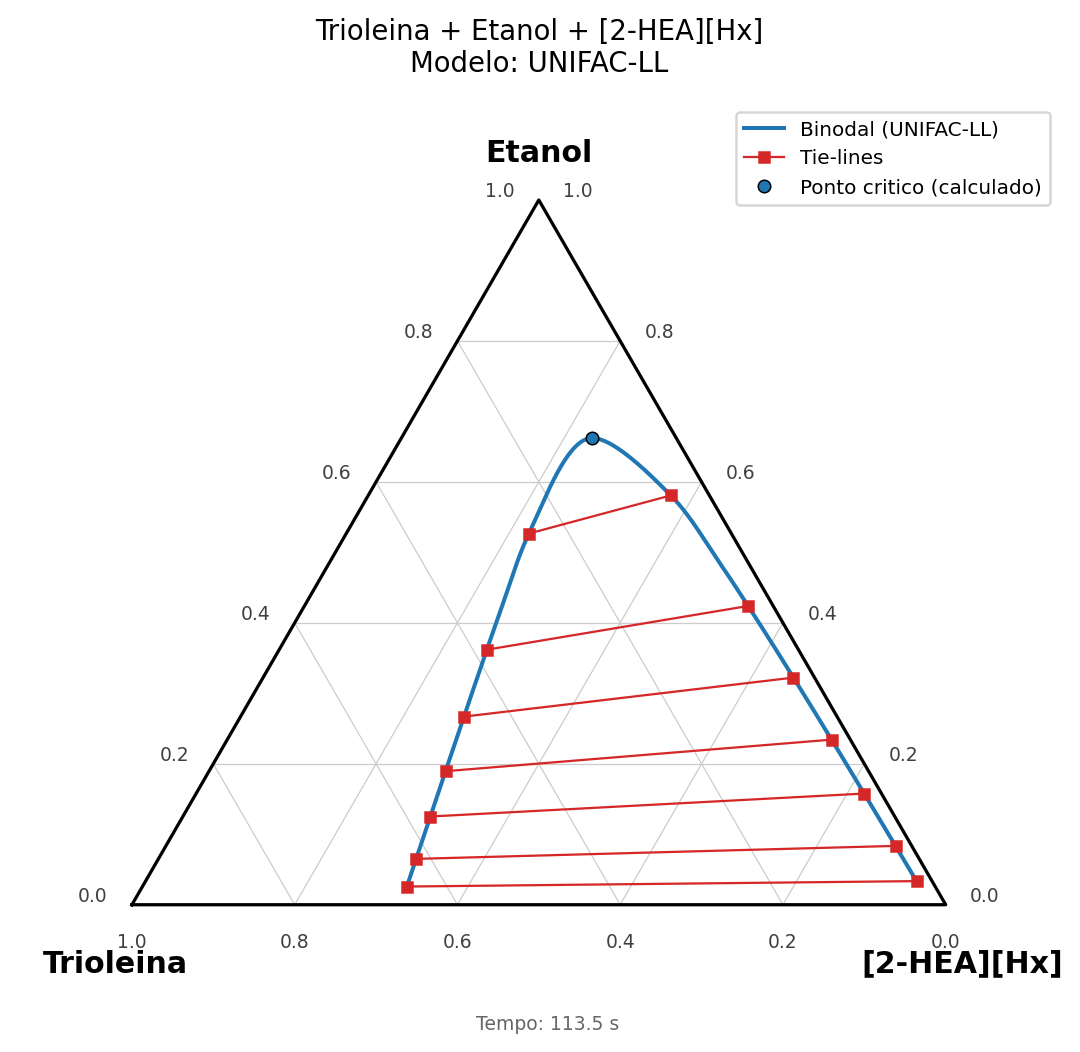
\includegraphics[width=0.4\textwidth]{imagens/ELL_Trioleina_Etanol_2_HEAHx_UNIFAC_LL.png}
\hfill
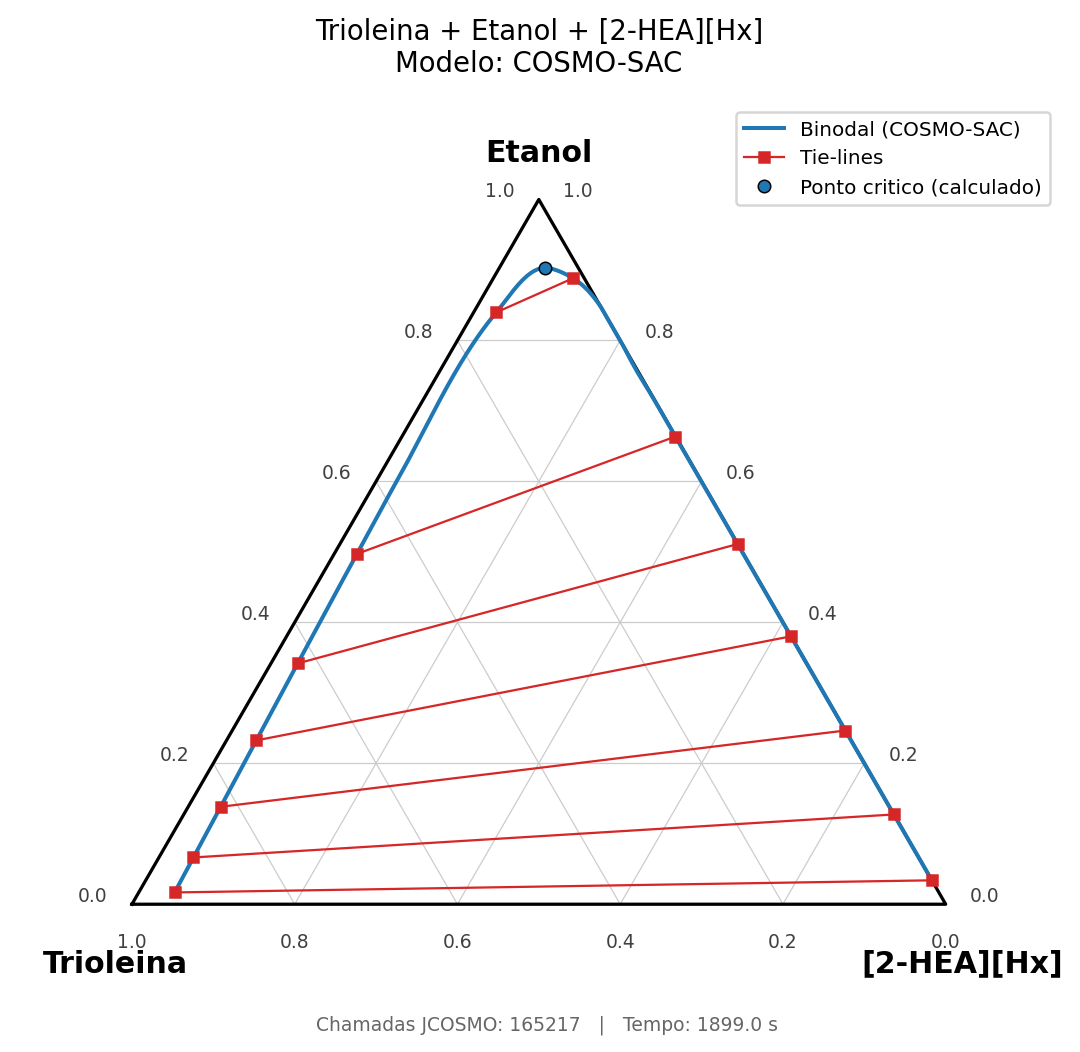
\includegraphics[width=0.4\textwidth]{imagens/ELL_Trioleina_Etanol_2_HEAHx_COSMO_SAC.png}
\caption{Trioleína + etanol + [2-HEA][Hx]: UNIFAC-LL (esquerda) e COSMO-SAC (direita)}
\label{fig:trioleina_etanol_2hea}
\end{figure}

\begin{figure}[H]
\centering
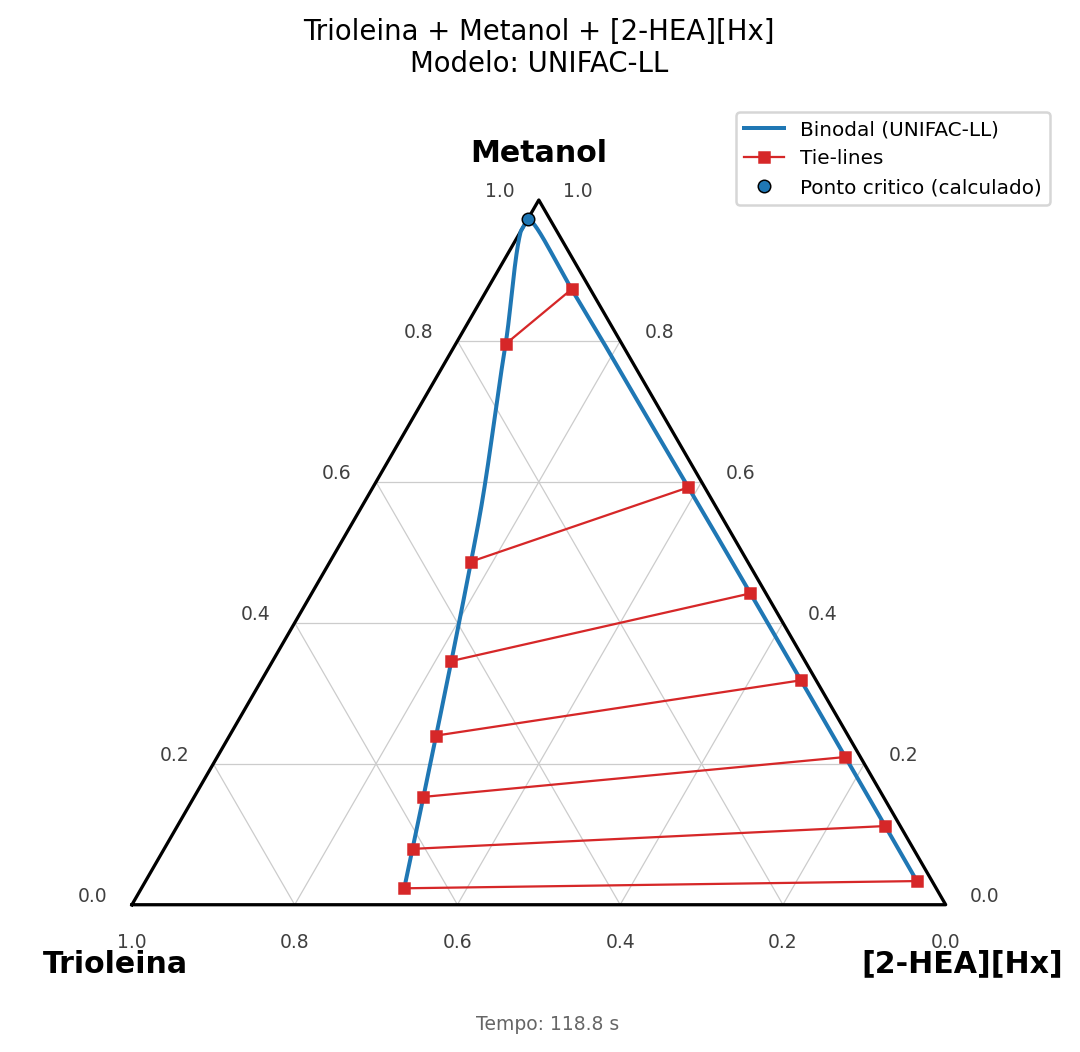
\includegraphics[width=0.4\textwidth]{imagens/ELL_Trioleina_Metanol_2_HEAHx_UNIFAC_LL.png}
\hfill
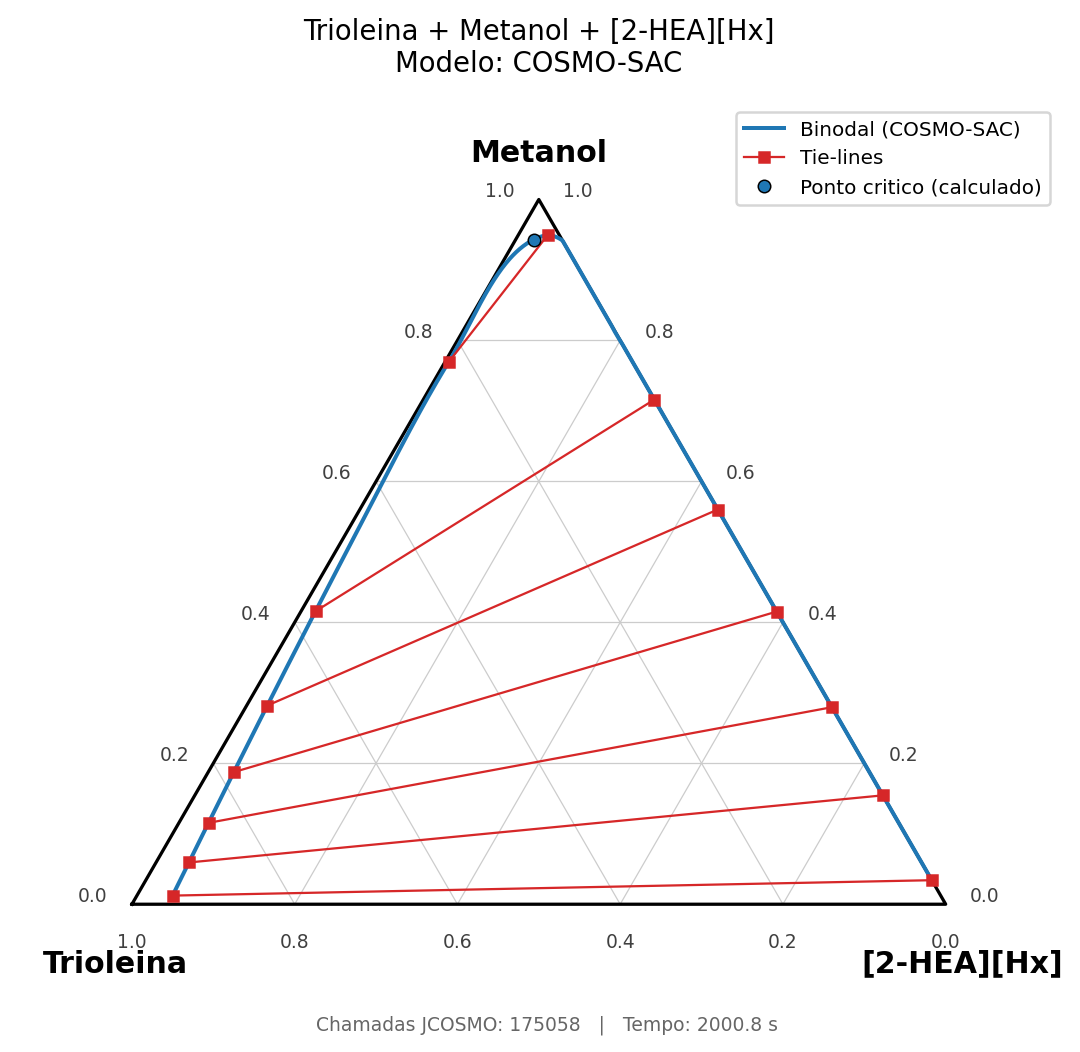
\includegraphics[width=0.4\textwidth]{imagens/ELL_Trioleina_Metanol_2_HEAHx_COSMO_SAC.png}
\caption{Trioleína + metanol + [2-HEA][Hx]: UNIFAC-LL (esquerda) e COSMO-SAC (direita)}
\label{fig:trioleina_metanol_2hea}
\end{figure}

\begin{figure}[H]
\centering
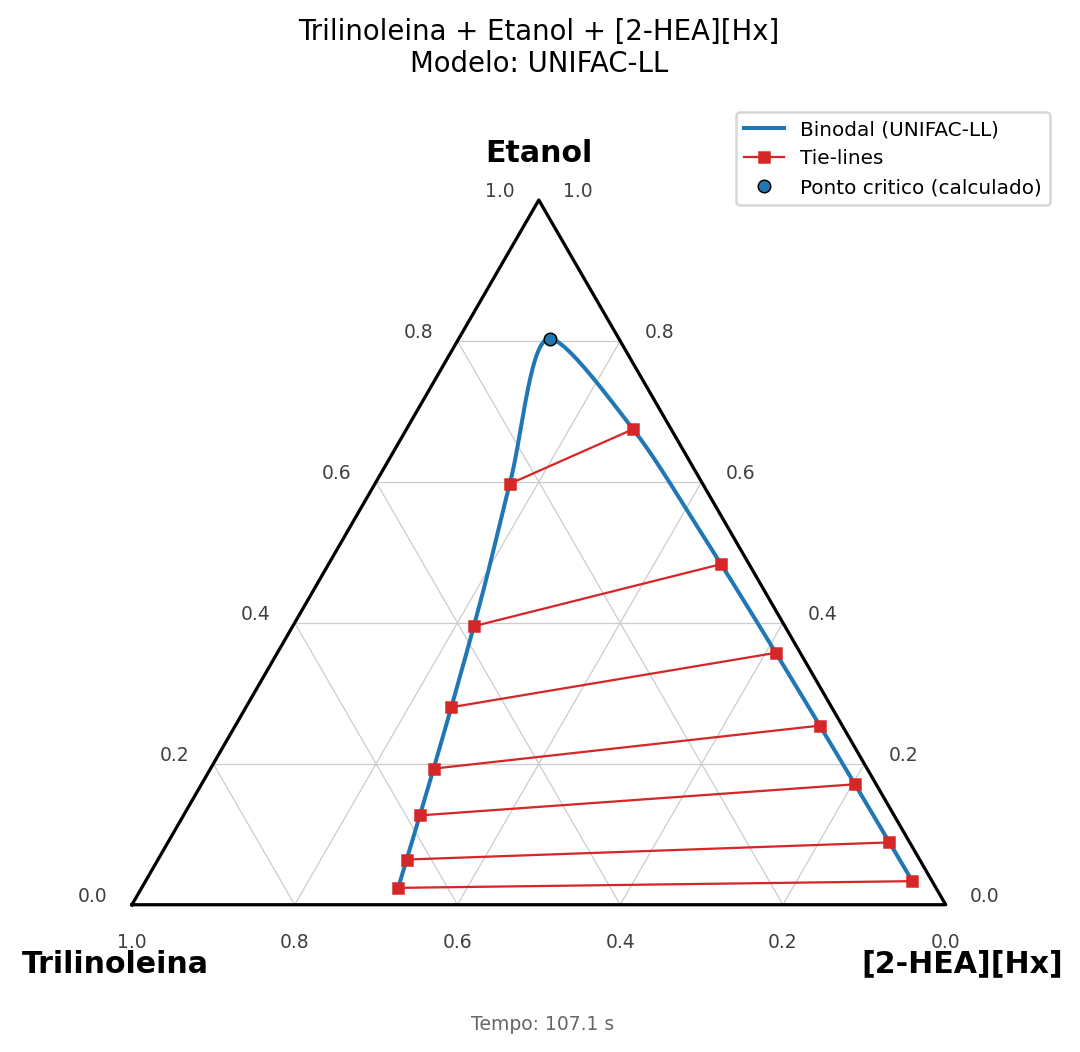
\includegraphics[width=0.4\textwidth]{imagens/ELL_Trilinoleina_Etanol_2_HEAHx_UNIFAC_LL.png}
\hfill
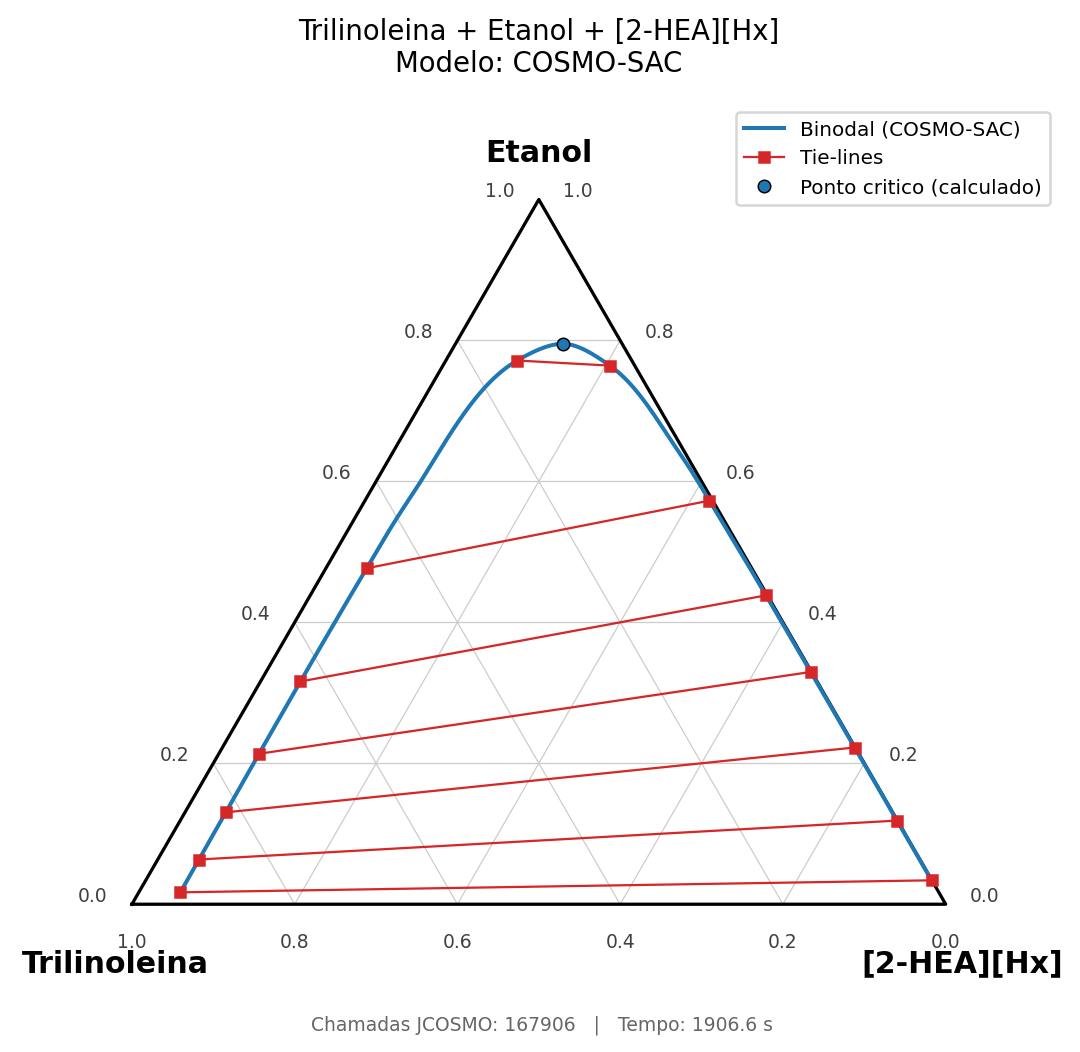
\includegraphics[width=0.4\textwidth]{imagens/ELL_Trilinoleina_Etanol_2_HEAHx_COSMO_SAC.png}
\caption{Trilinoleína + etanol + [2-HEA][Hx]: UNIFAC-LL (esquerda) e COSMO-SAC (direita)}
\label{fig:trilinoleina_etanol_2hea}
\end{figure}

\begin{figure}[H]
\centering
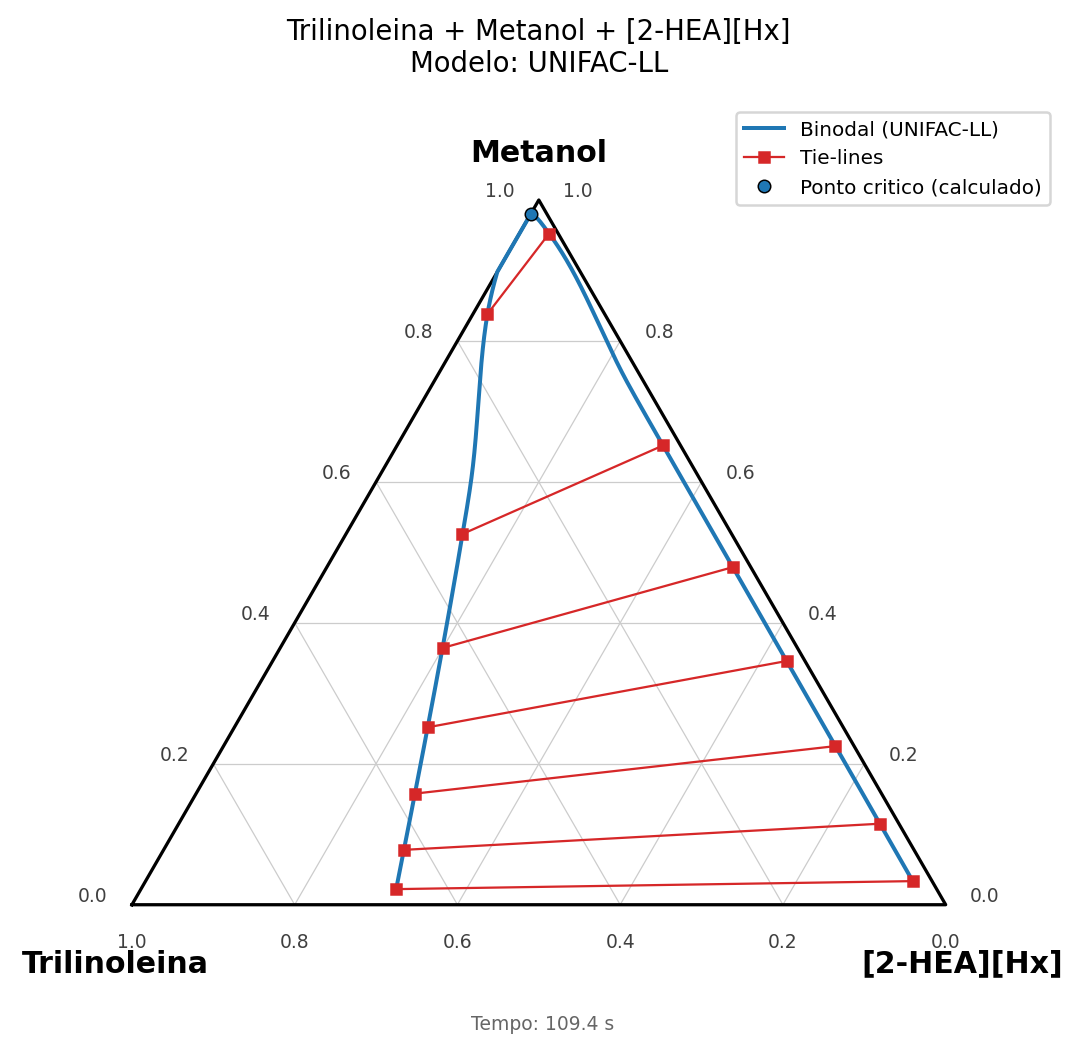
\includegraphics[width=0.4\textwidth]{imagens/ELL_Trilinoleina_Metanol_2_HEAHx_UNIFAC_LL.png}
\hfill
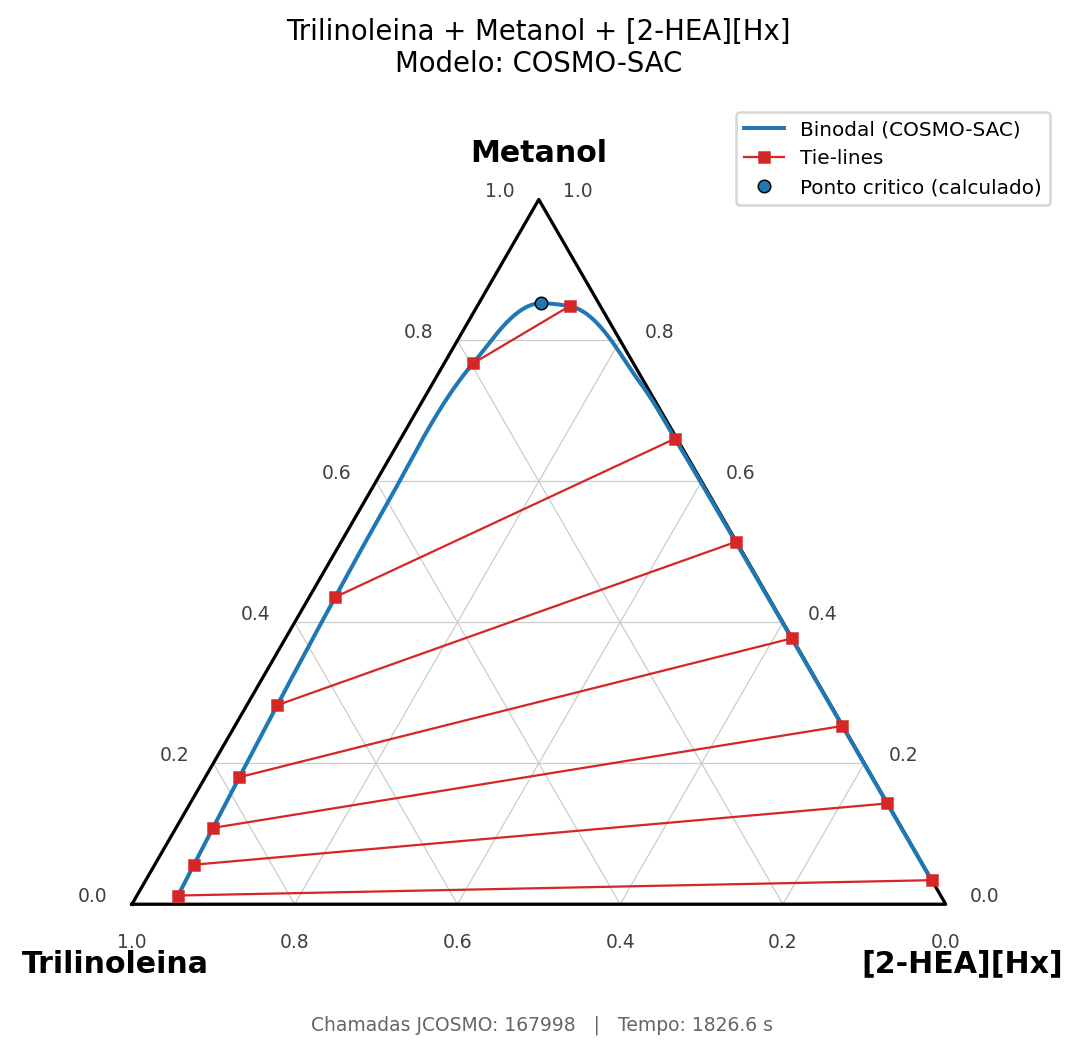
\includegraphics[width=0.4\textwidth]{imagens/ELL_Trilinoleina_Metanol_2_HEAHx_COSMO_SAC.png}
\caption{Trilinoleína + metanol + [2-HEA][Hx]: UNIFAC-LL (esquerda) e COSMO-SAC (direita)}
\label{fig:trilinoleina_metanol_2hea}
\end{figure}

\begin{figure}[H]
\centering
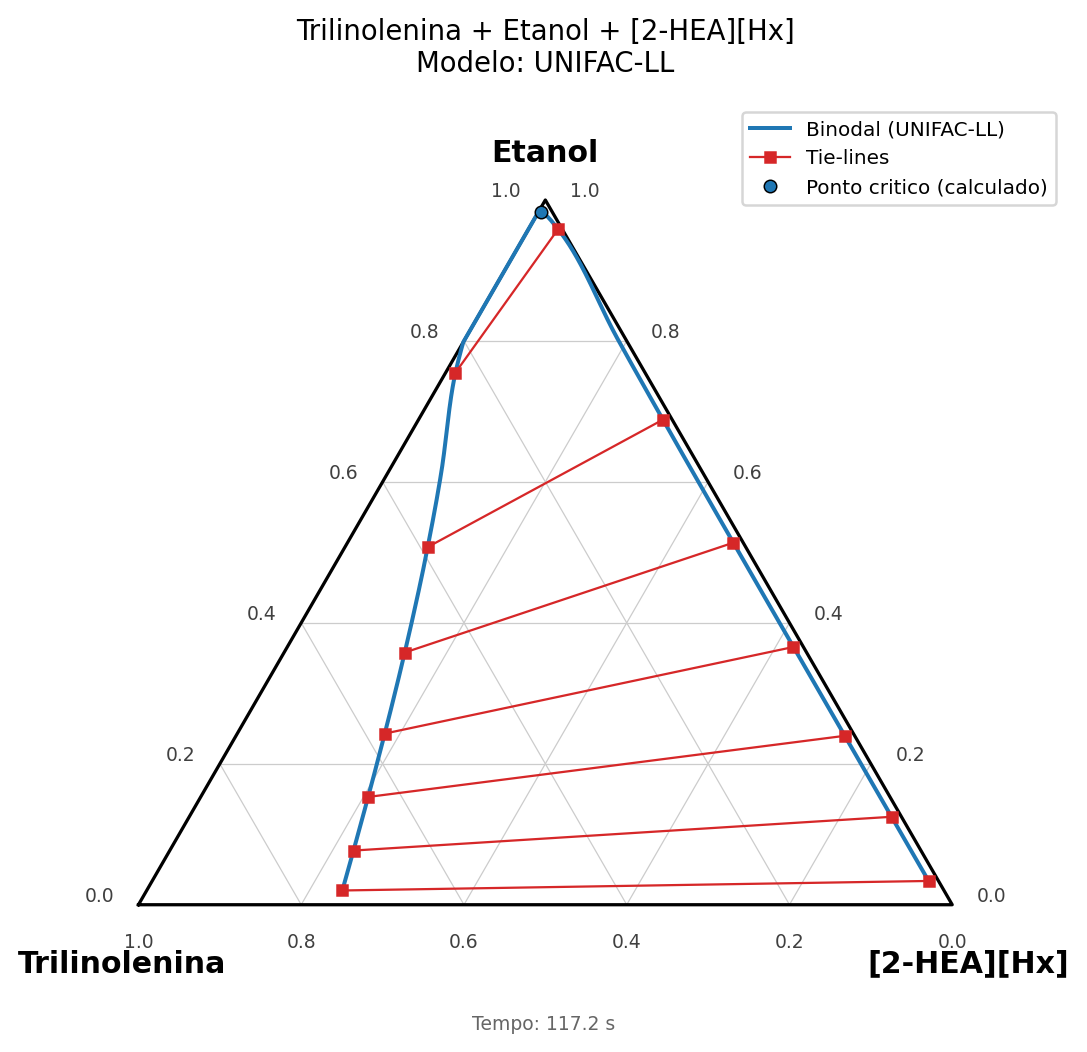
\includegraphics[width=0.4\textwidth]{imagens/ELL_Trilinolenina_Etanol_2_HEAHx_UNIFAC_LL.png}
\hfill
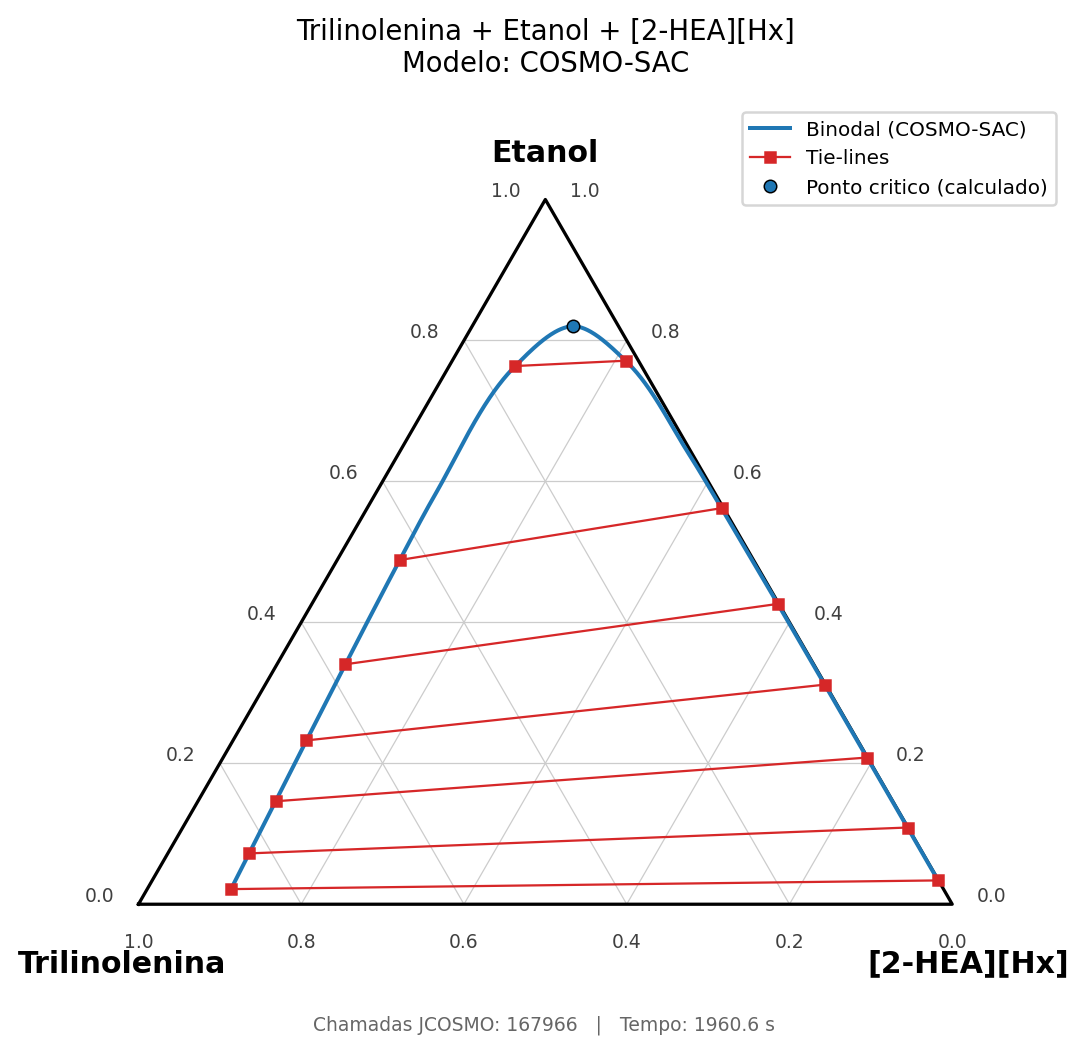
\includegraphics[width=0.4\textwidth]{imagens/ELL_Trilinolenina_Etanol_2_HEAHx_COSMO_SAC.png}
\caption{Trilinolenina + etanol + [2-HEA][Hx]: UNIFAC-LL (esquerda) e COSMO-SAC (direita)}
\label{fig:trilinolenina_etanol_2hea}
\end{figure}

\begin{figure}[H]
\centering
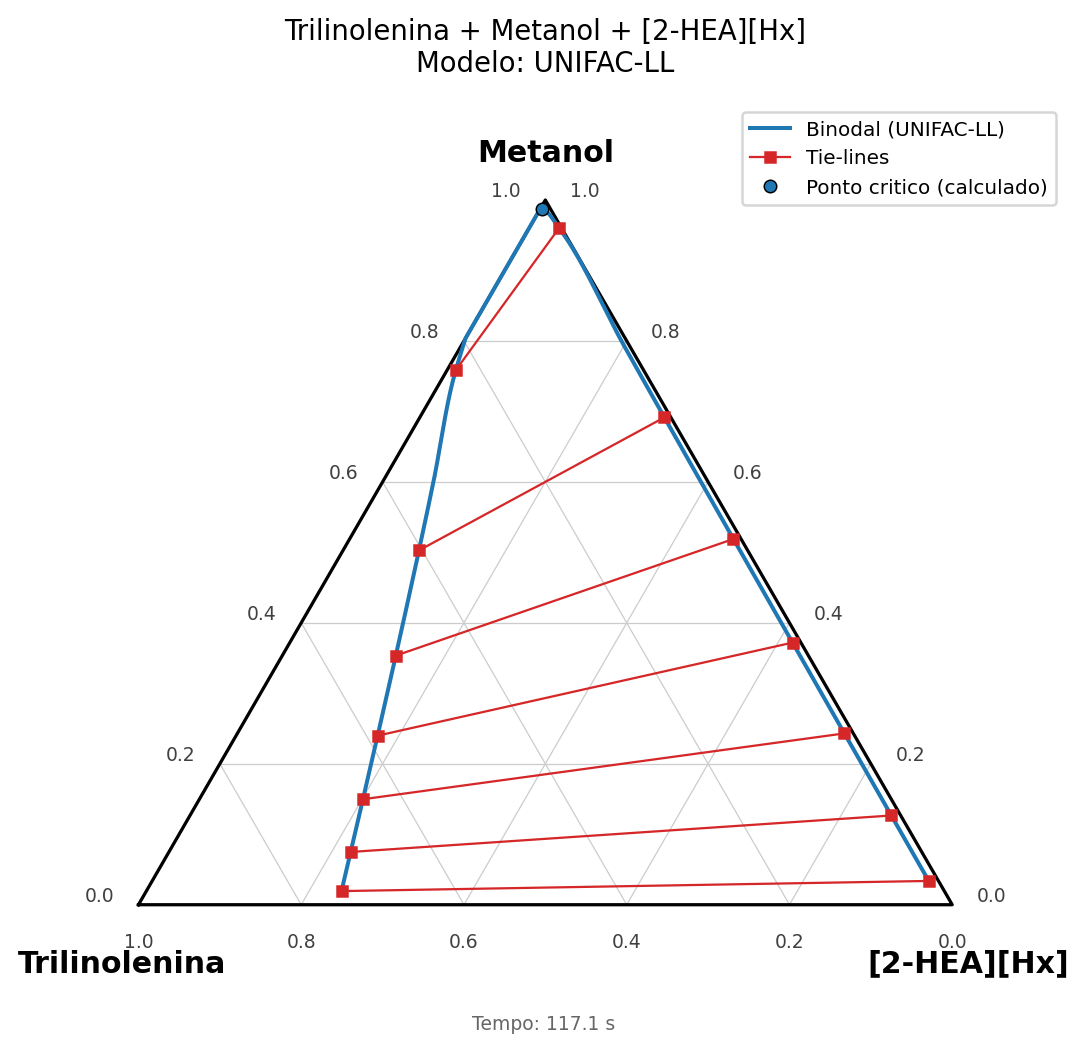
\includegraphics[width=0.4\textwidth]{imagens/ELL_Trilinolenina_Metanol_2_HEAHx_UNIFAC_LL.png}
\hfill
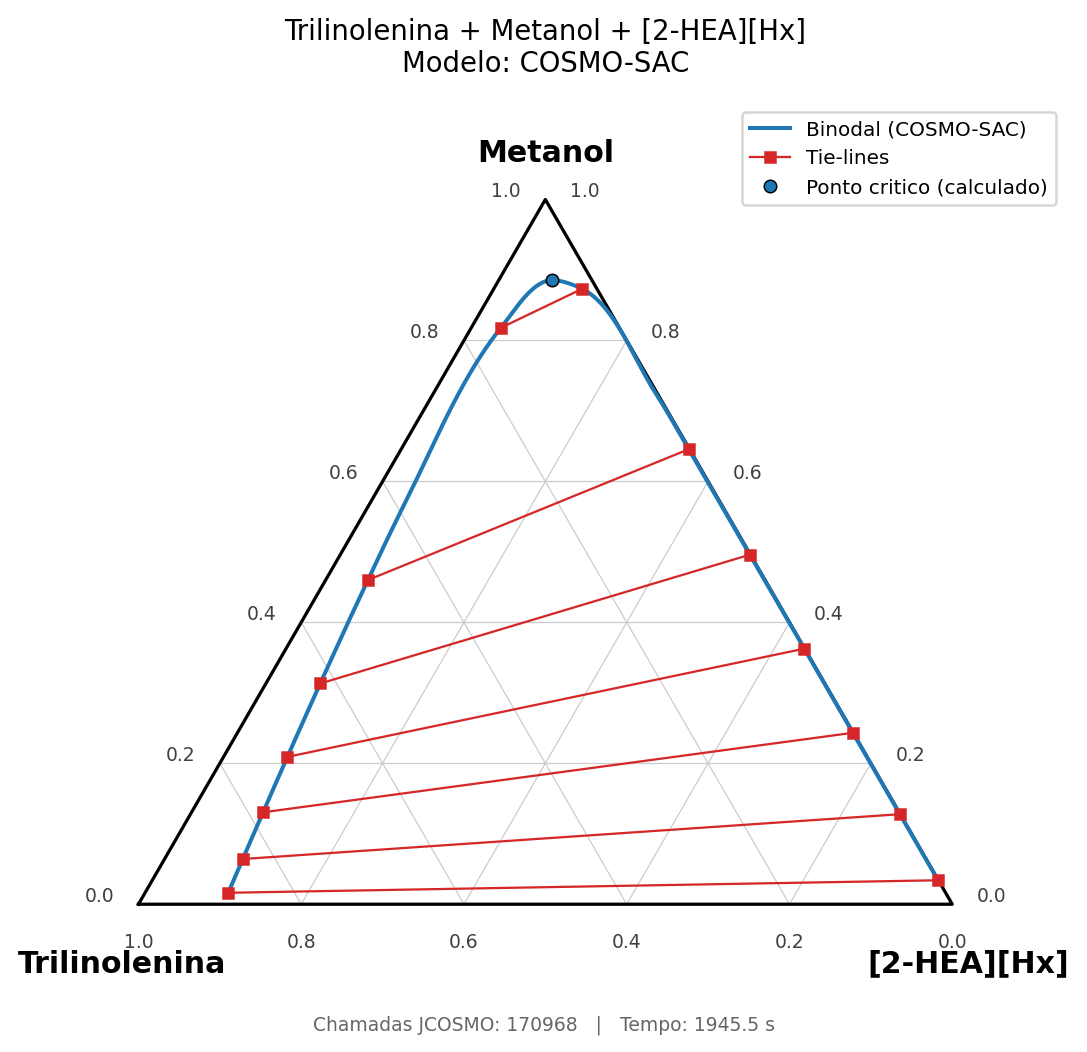
\includegraphics[width=0.4\textwidth]{imagens/ELL_Trilinolenina_Metanol_2_HEAHx_COSMO_SAC.png}
\caption{Trilinolenina + metanol + [2-HEA][Hx]: UNIFAC-LL (esquerda) e COSMO-SAC (direita)}
\label{fig:trilinolenina_metanol_2hea}
\end{figure}

Quanto à extensão da região bifásica, a área calculada pelo COSMO-SAC varia entre 0,3819 e 0,4564 nesses seis sistemas (média de 0,4214), faixa retomada adiante na comparação com os sistemas contendo [DETA][Hx] (Seção~\ref{subsec:resultados_deta}). A concordância entre os dois modelos, nesse conjunto, é de natureza qualitativa, pois ambos preveem o mesmo tipo de binodal e não divergem quanto à existência de duas fases líquidas, embora posicionem a curva de maneira distinta no espaço de composições. Tal distinção pode ser medida pela distância euclidiana entre os pontos críticos estimados por cada modelo para um mesmo sistema, que se situa entre 0,0616 e 0,3966 em fração molar (média de 0,1599), com o sistema \{trioleína + etanol\} destacando-se dos demais ao registrar a maior distância (0,3966) enquanto os outros cinco permanecem entre 0,0616 e 0,1621. Uma vez que o ponto crítico é obtido por extrapolação do encolhimento sucessivo da região instável (Seção~\ref{subsec:motor_termodinamico}), em vez de resolver-se diretamente a condição crítica, essas distâncias carregam a incerteza própria desse procedimento e devem ser lidas como ordem de grandeza da discrepância entre os modelos.

Considerando-se que os dois modelos partem de naturezas bastante distintas (contribuição de grupos, de um lado, e cálculo a priori a partir de perfis sigma, de outro), a coincidência quanto ao tipo de comportamento de fases sugere que a tendência à separação nos sistemas com [2-HEA][Hx] não depende da escolha de um modelo específico, ainda que a verificação dessa leitura dependa de dados experimentais indisponíveis para esses sistemas (Seção~\ref{sec:dados_validacao}).

Entre os três triglicerídeos, o resultado da trilinoleína deve ser lido com a ressalva já registrada na Seção~\ref{subsec:parametros_perfis}, visto que o enovelamento identificado em seu perfil sigma tende a superestimar a fração polar da molécula e, por conseguinte, sua afinidade com o álcool e com o líquido iônico. Como apenas o COSMO-SAC consome o perfil sigma comprometido, a formação de região bifásica também no UNIFAC-LL, que não depende dessa geometria, indica que o comportamento em si não decorre exclusivamente do artefato.

\subsection{Sistemas com [DETA][Hx]}
\label{subsec:resultados_deta}

Os sistemas que envolvem o líquido iônico prótico [DETA][Hx] apresentam um quadro distinto do anterior, no qual os dois modelos deixam de concordar sequer quanto à existência de duas fases líquidas. No UNIFAC-LL, nenhum dos seis sistemas apresentou binodal genuína, uma vez que os quatro casos com trioleína e trilinoleína convergiram diretamente para zero linhas de amarração, ou seja, o teste de estabilidade não identificou composição instável em toda a extensão do diagrama, enquanto os dois casos com trilinolenina produziram apenas quatro linhas, confinadas a uma faixa estreita próxima ao vértice do álcool puro (fração de trilinolenina inferior a 0,23 em ambas as fases). Não foi possível, portanto, construir a curva binodal para nenhum dos seis sistemas com [DETA][Hx] no UNIFAC-LL, e o resultado é registrado nesses termos, já que a ausência de composição instável identificada pelo teste de estabilidade é compatível tanto com uma fase única termodinamicamente estável quanto com uma falha de convergência do procedimento nas condições avaliadas.

O COSMO-SAC, em contrapartida, prevê binodal do tipo 1 em todos os seis, com número de linhas de amarração entre 327 e 370 (Tabela~\ref{tab:tielines_deta}), na mesma ordem de grandeza registrada para os sistemas com [2-HEA][Hx].

\begin{table}[htb]
\centering
\caption{Número de tie-lines calculadas para os sistemas com [DETA][Hx]}
\label{tab:tielines_deta}
\begin{tabular}{lcc}
\hline
Sistema & UNIFAC-LL & COSMO-SAC \\
\hline
Trioleína + Etanol      & 0 (curva não obtida) & 367 \\
Trioleína + Metanol     & 0 (curva não obtida) & 362 \\
Trilinoleína + Etanol   & 0 (curva não obtida) & 370 \\
Trilinoleína + Metanol  & 0 (curva não obtida) & 356 \\
Trilinolenina + Etanol  & 4 (insuficientes para a curva) & 334 \\
Trilinolenina + Metanol & 4 (insuficientes para a curva) & 344 \\
\hline
\end{tabular}
\end{table}

\begin{figure}[H]
\centering
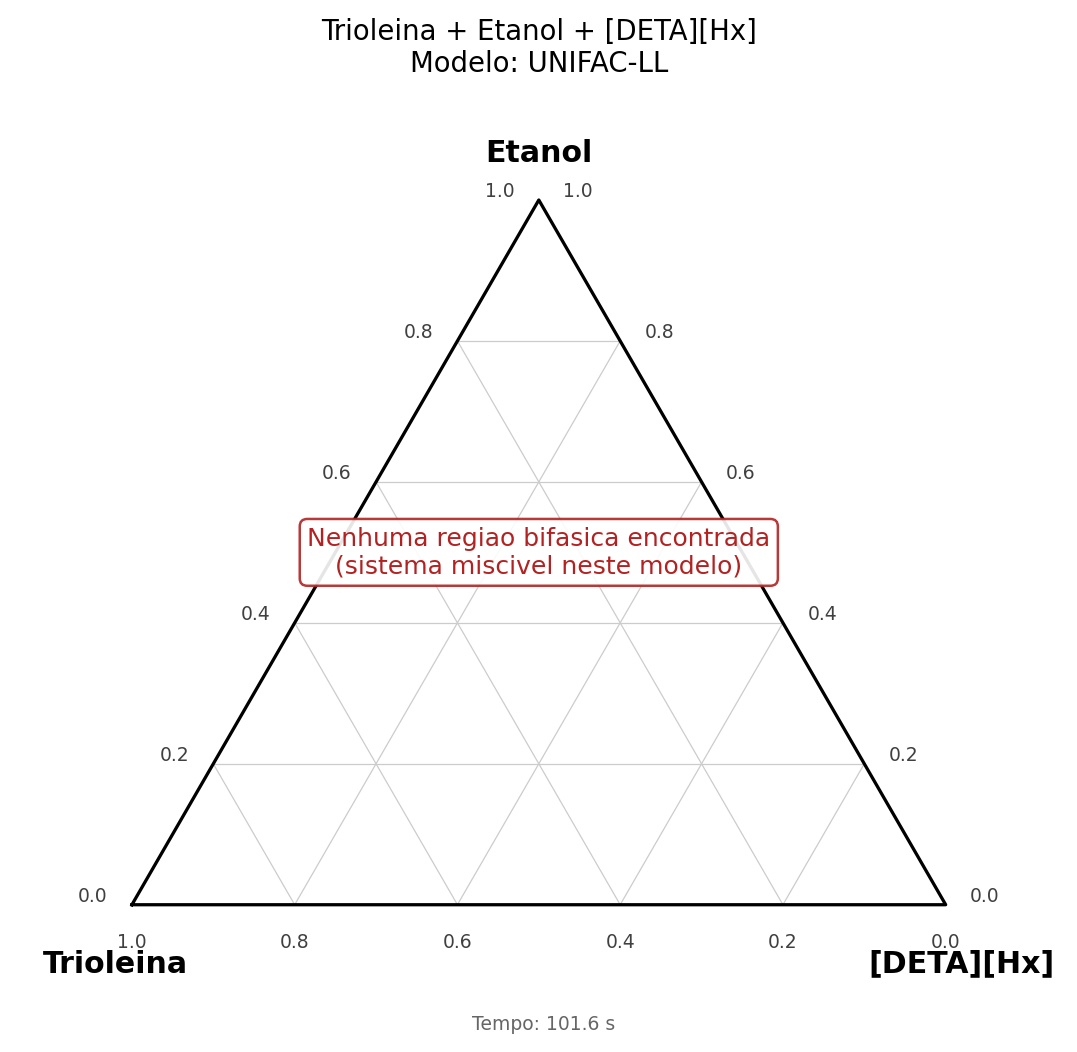
\includegraphics[width=0.4\textwidth]{imagens/ELL_Trioleina_Etanol_DETAHx_UNIFAC_LL.png}
\hfill
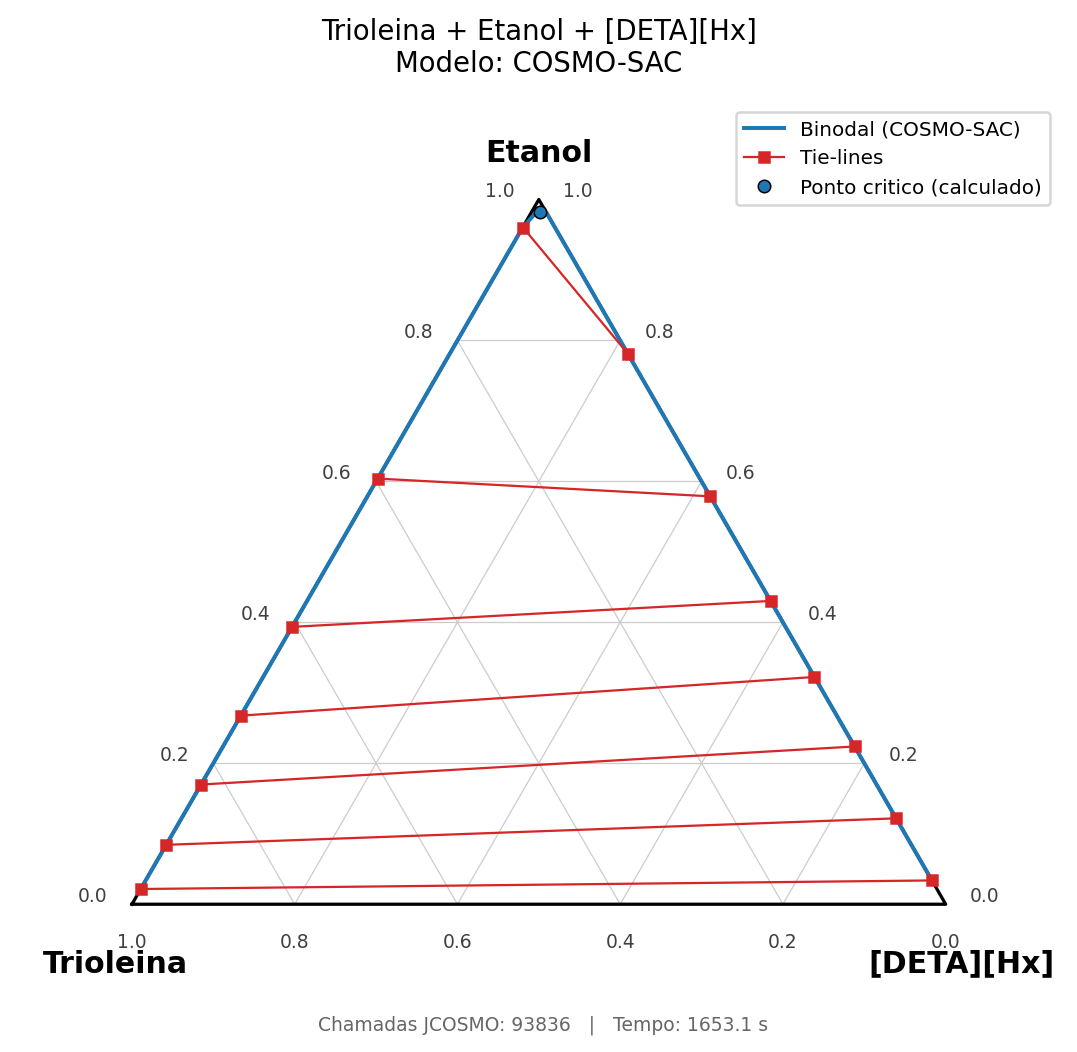
\includegraphics[width=0.4\textwidth]{imagens/ELL_Trioleina_Etanol_DETAHx_COSMO_SAC.png}
\caption{Trioleína + etanol + [DETA][Hx]: UNIFAC-LL (esquerda, curva não obtida) e COSMO-SAC (direita)}
\label{fig:trioleina_etanol_deta}
\end{figure}

\begin{figure}[H]
\centering
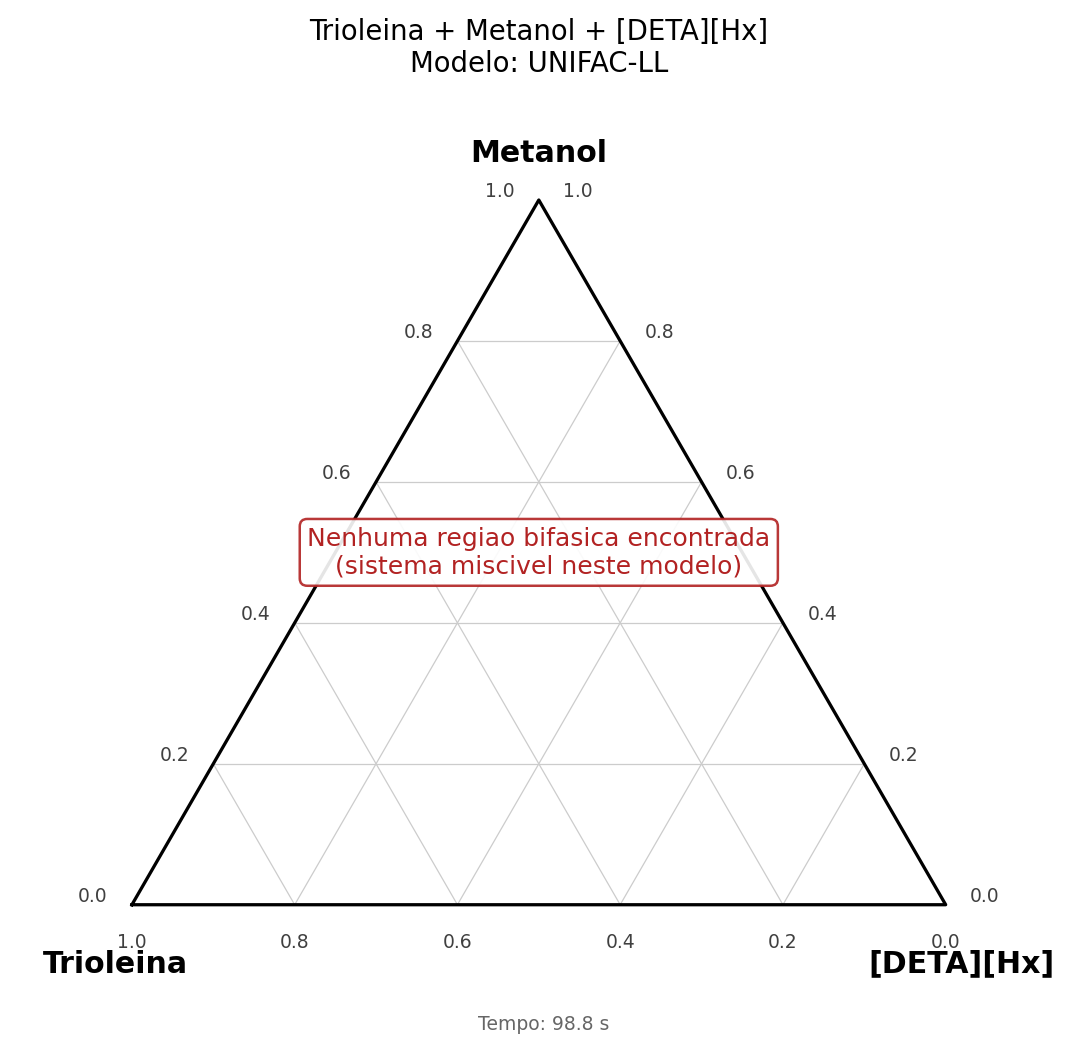
\includegraphics[width=0.4\textwidth]{imagens/ELL_Trioleina_Metanol_DETAHx_UNIFAC_LL.png}
\hfill
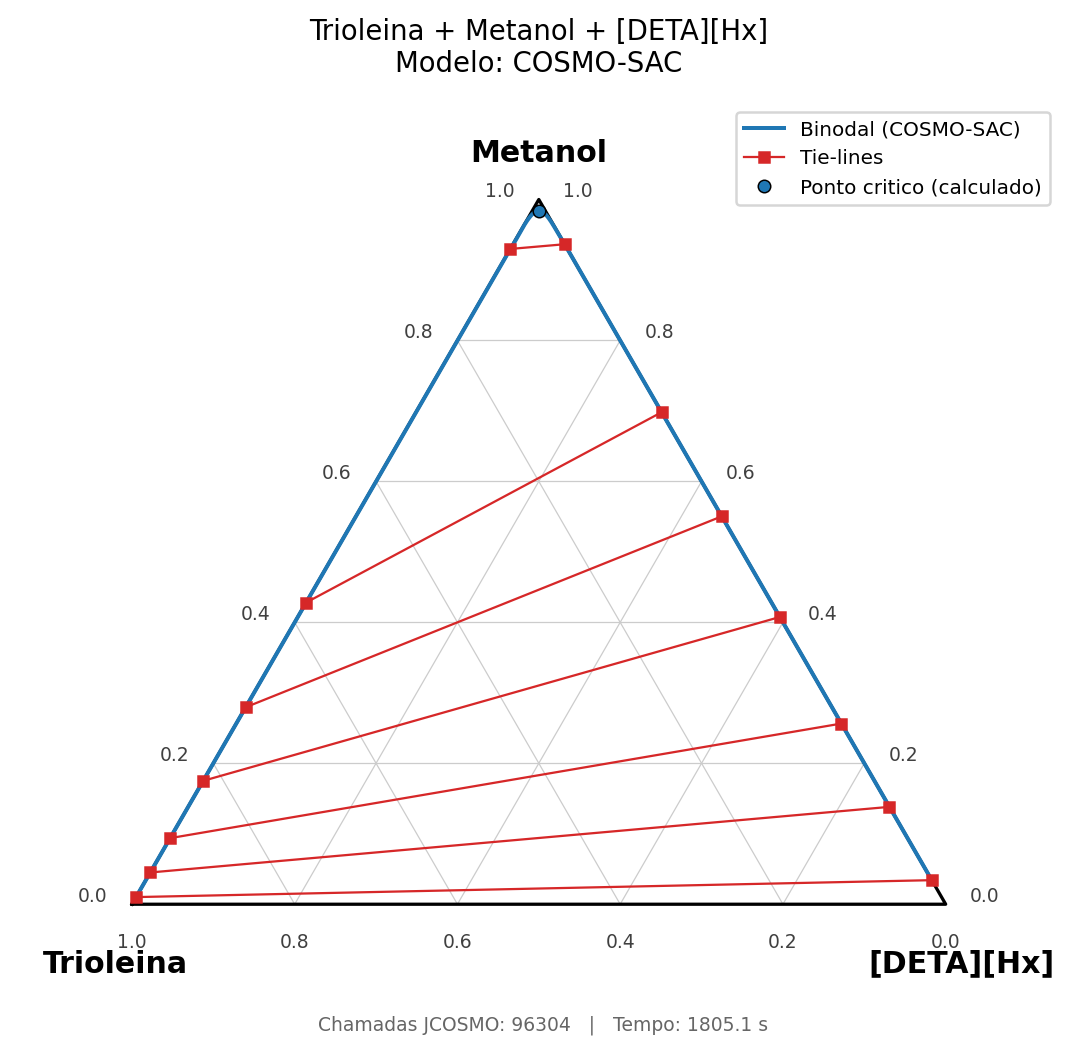
\includegraphics[width=0.4\textwidth]{imagens/ELL_Trioleina_Metanol_DETAHx_COSMO_SAC.png}
\caption{Trioleína + metanol + [DETA][Hx]: UNIFAC-LL (esquerda, curva não obtida) e COSMO-SAC (direita)}
\label{fig:trioleina_metanol_deta}
\end{figure}

\begin{figure}[H]
\centering
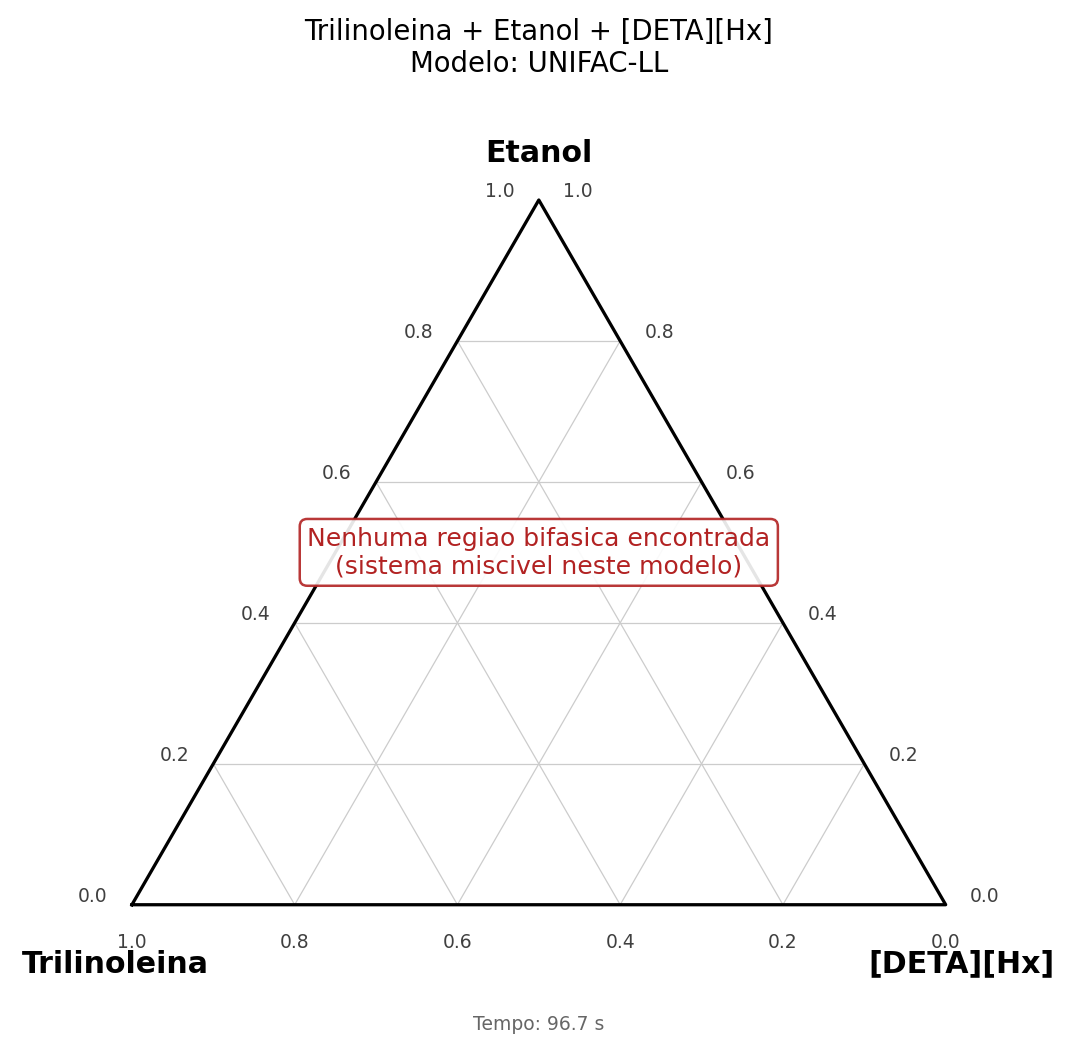
\includegraphics[width=0.4\textwidth]{imagens/ELL_Trilinoleina_Etanol_DETAHx_UNIFAC_LL.png}
\hfill
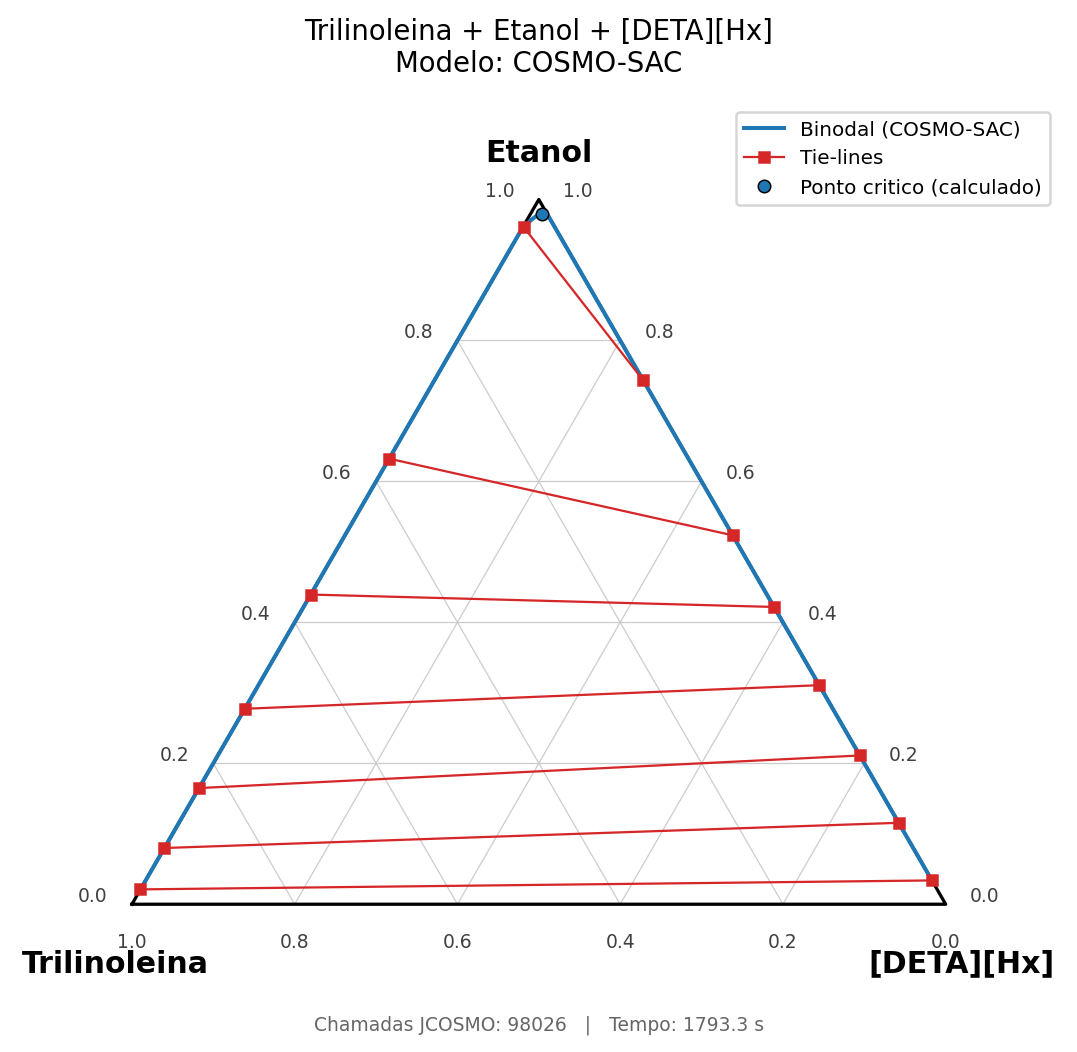
\includegraphics[width=0.4\textwidth]{imagens/ELL_Trilinoleina_Etanol_DETAHx_COSMO_SAC.png}
\caption{Trilinoleína + etanol + [DETA][Hx]: UNIFAC-LL (esquerda, curva não obtida) e COSMO-SAC (direita)}
\label{fig:trilinoleina_etanol_deta}
\end{figure}

\begin{figure}[H]
\centering
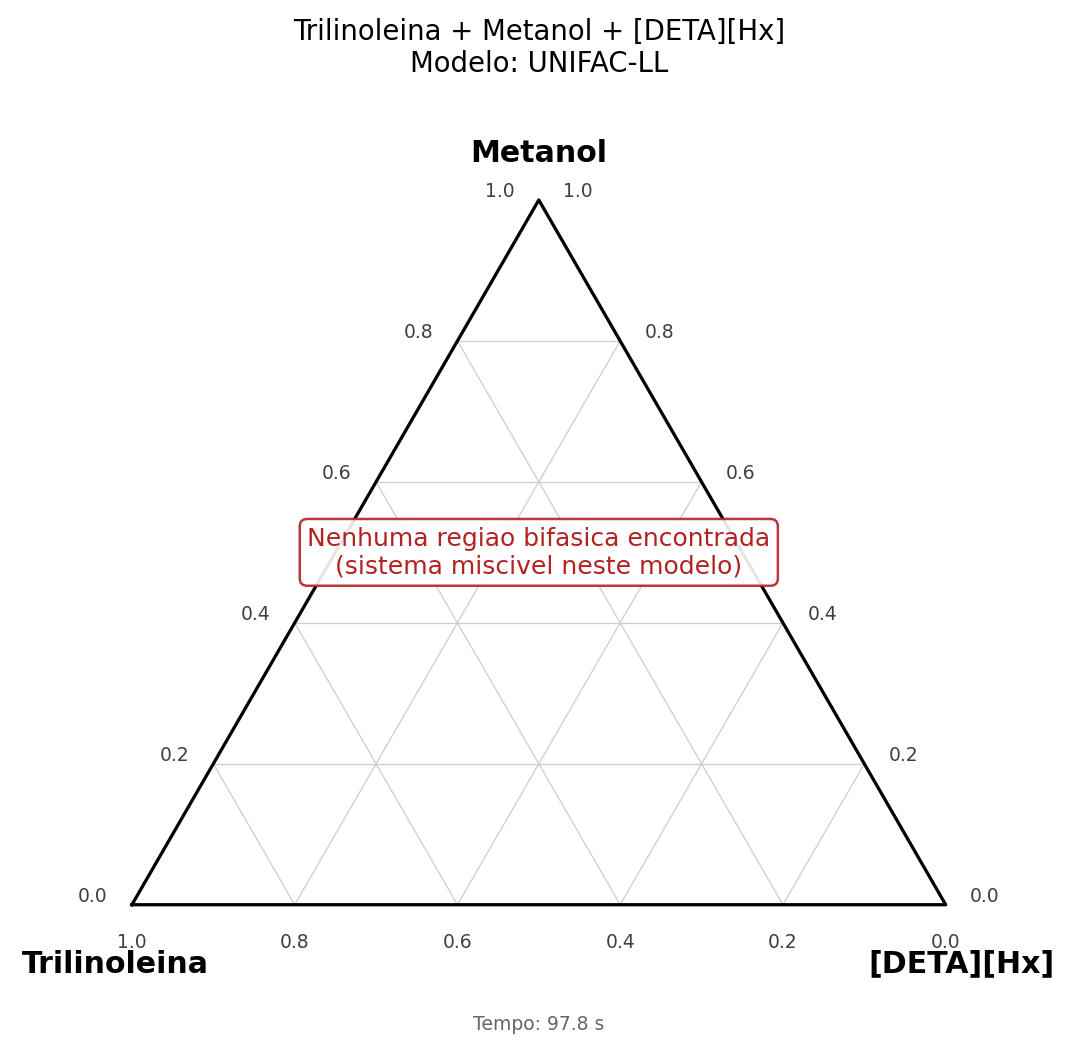
\includegraphics[width=0.4\textwidth]{imagens/ELL_Trilinoleina_Metanol_DETAHx_UNIFAC_LL.png}
\hfill
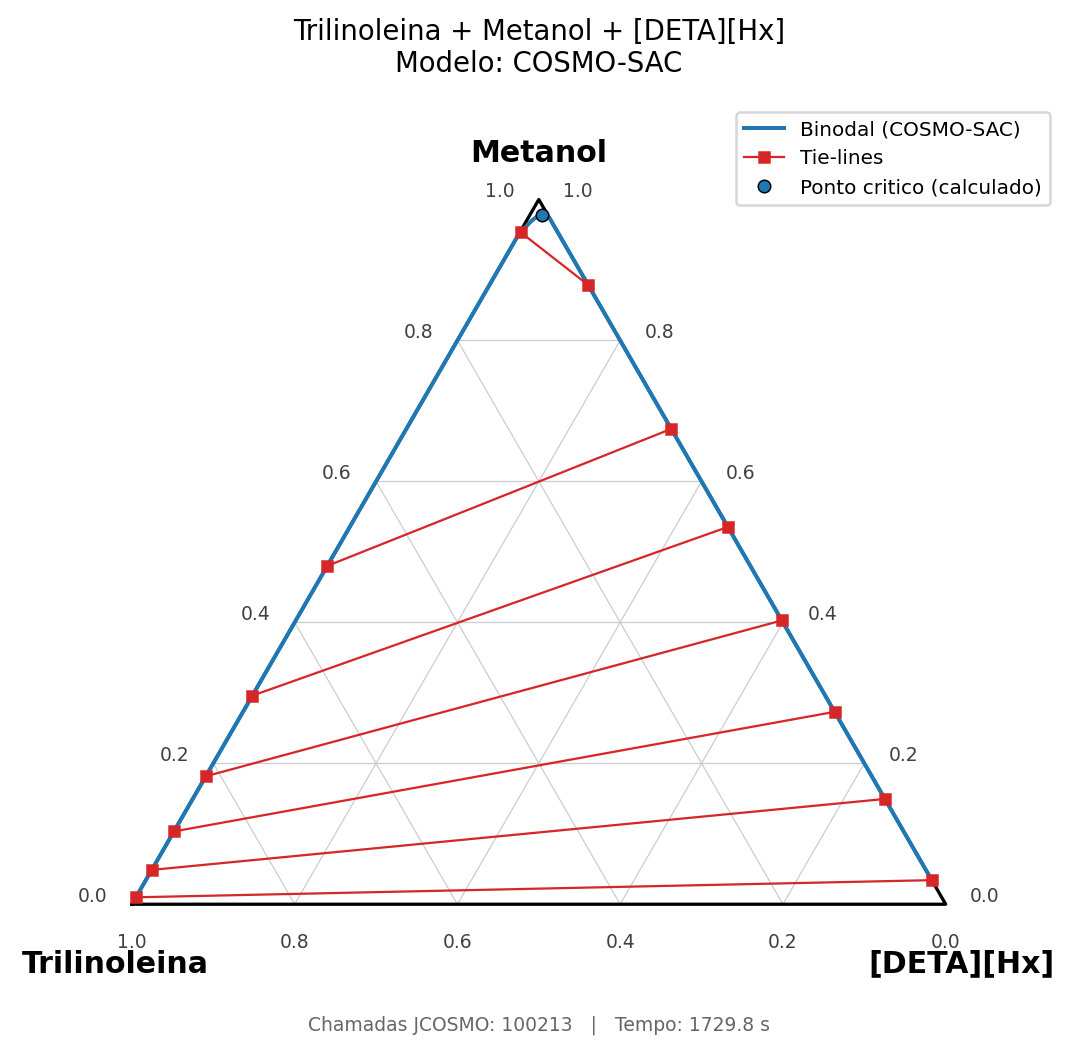
\includegraphics[width=0.4\textwidth]{imagens/ELL_Trilinoleina_Metanol_DETAHx_COSMO_SAC.png}
\caption{Trilinoleína + metanol + [DETA][Hx]: UNIFAC-LL (esquerda, curva não obtida) e COSMO-SAC (direita)}
\label{fig:trilinoleina_metanol_deta}
\end{figure}

\begin{figure}[H]
\centering
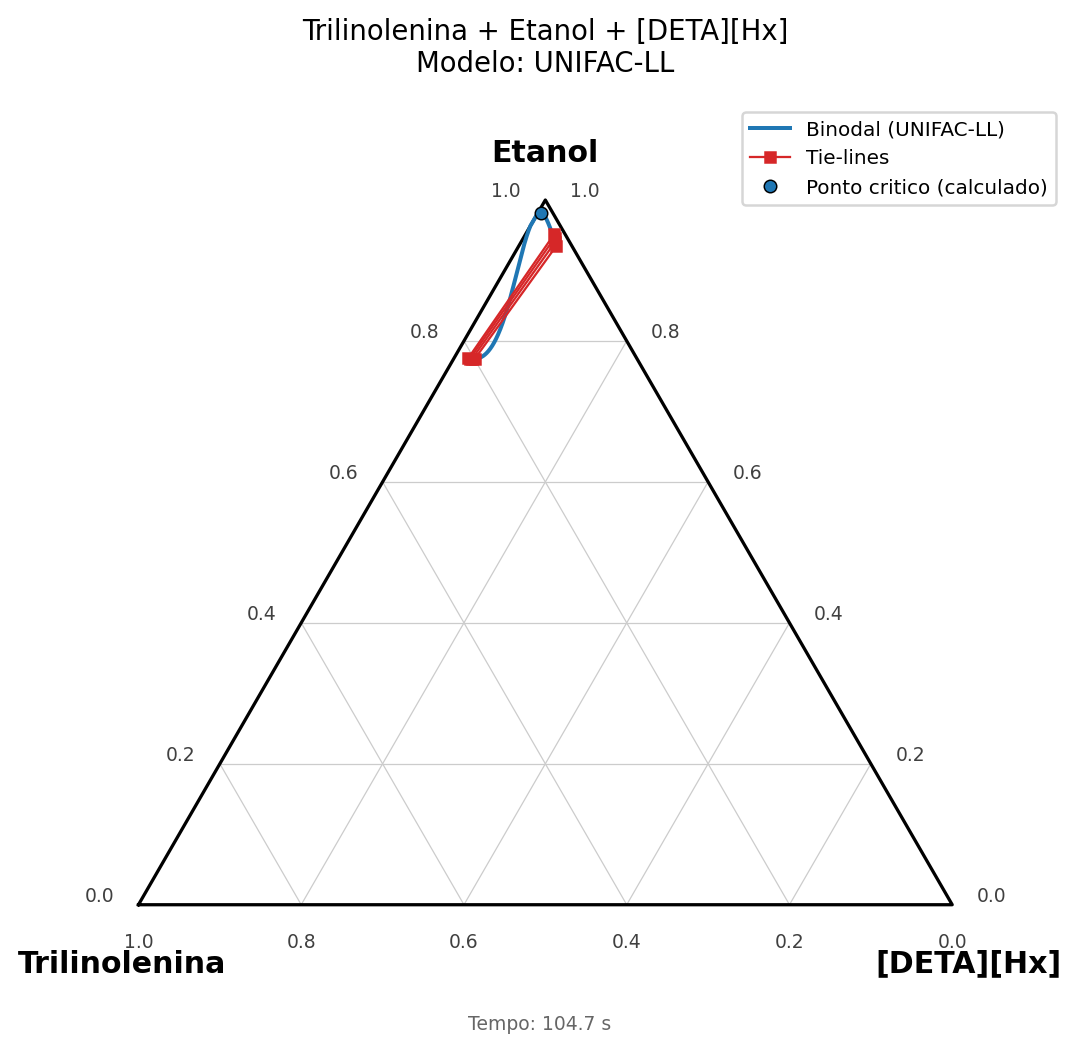
\includegraphics[width=0.4\textwidth]{imagens/ELL_Trilinolenina_Etanol_DETAHx_UNIFAC_LL.png}
\hfill
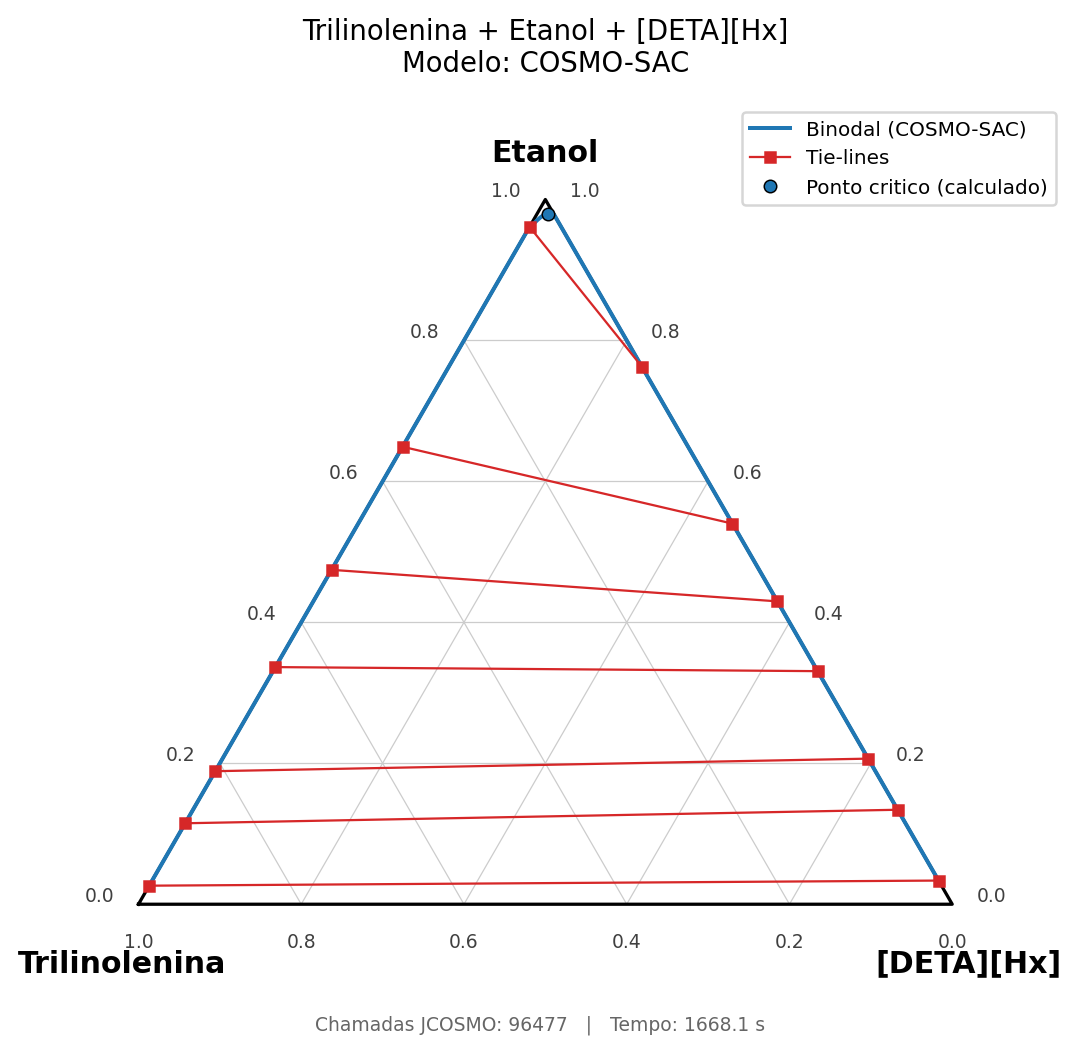
\includegraphics[width=0.4\textwidth]{imagens/ELL_Trilinolenina_Etanol_DETAHx_COSMO_SAC.png}
\caption{Trilinolenina + etanol + [DETA][Hx]: o UNIFAC-LL (esquerda) produz apenas quatro tie-lines confinadas ao vértice do álcool, insuficientes para o traçado da curva; o COSMO-SAC (direita) prevê uma binodal completa}
\label{fig:trilinolenina_etanol_deta}
\end{figure}

\begin{figure}[H]
\centering
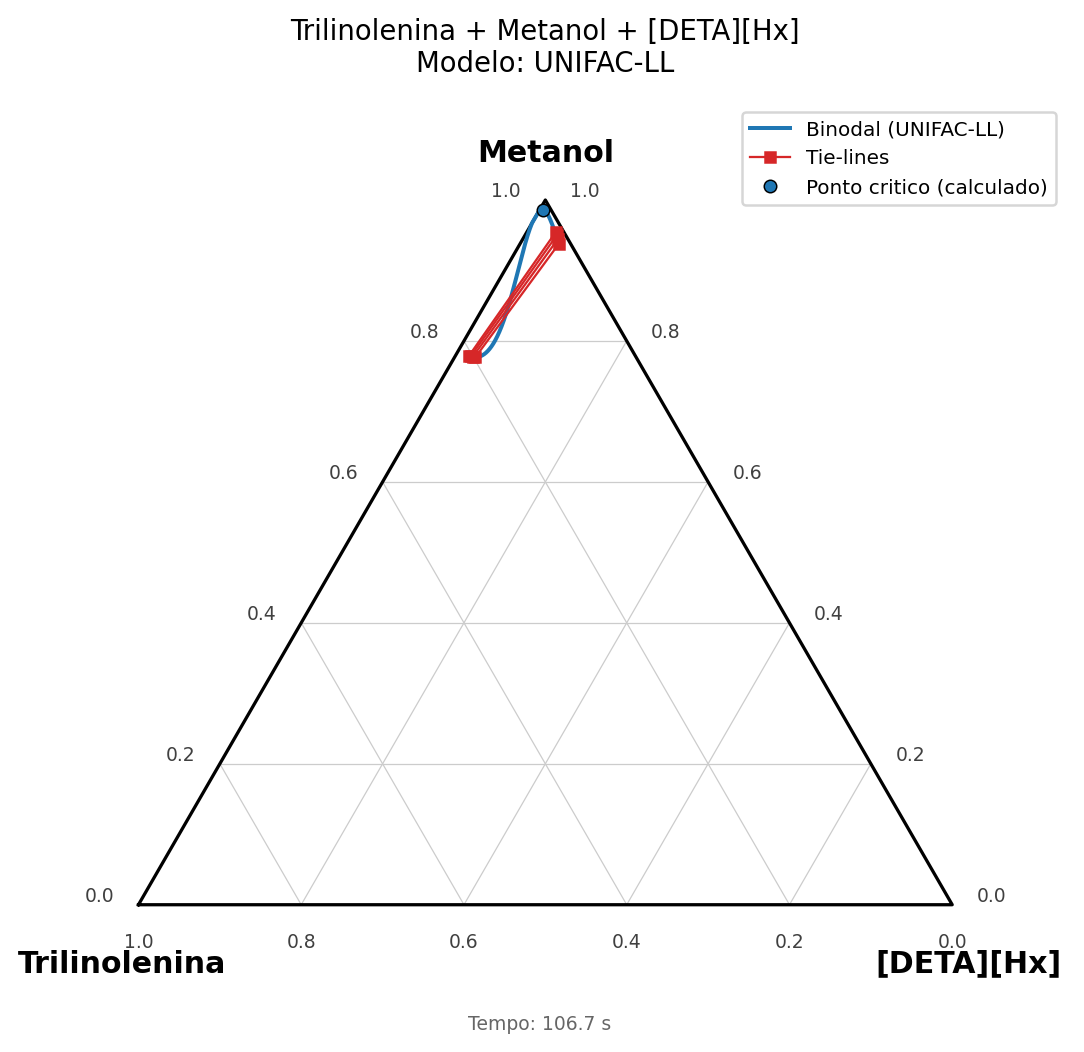
\includegraphics[width=0.4\textwidth]{imagens/ELL_Trilinolenina_Metanol_DETAHx_UNIFAC_LL.png}
\hfill
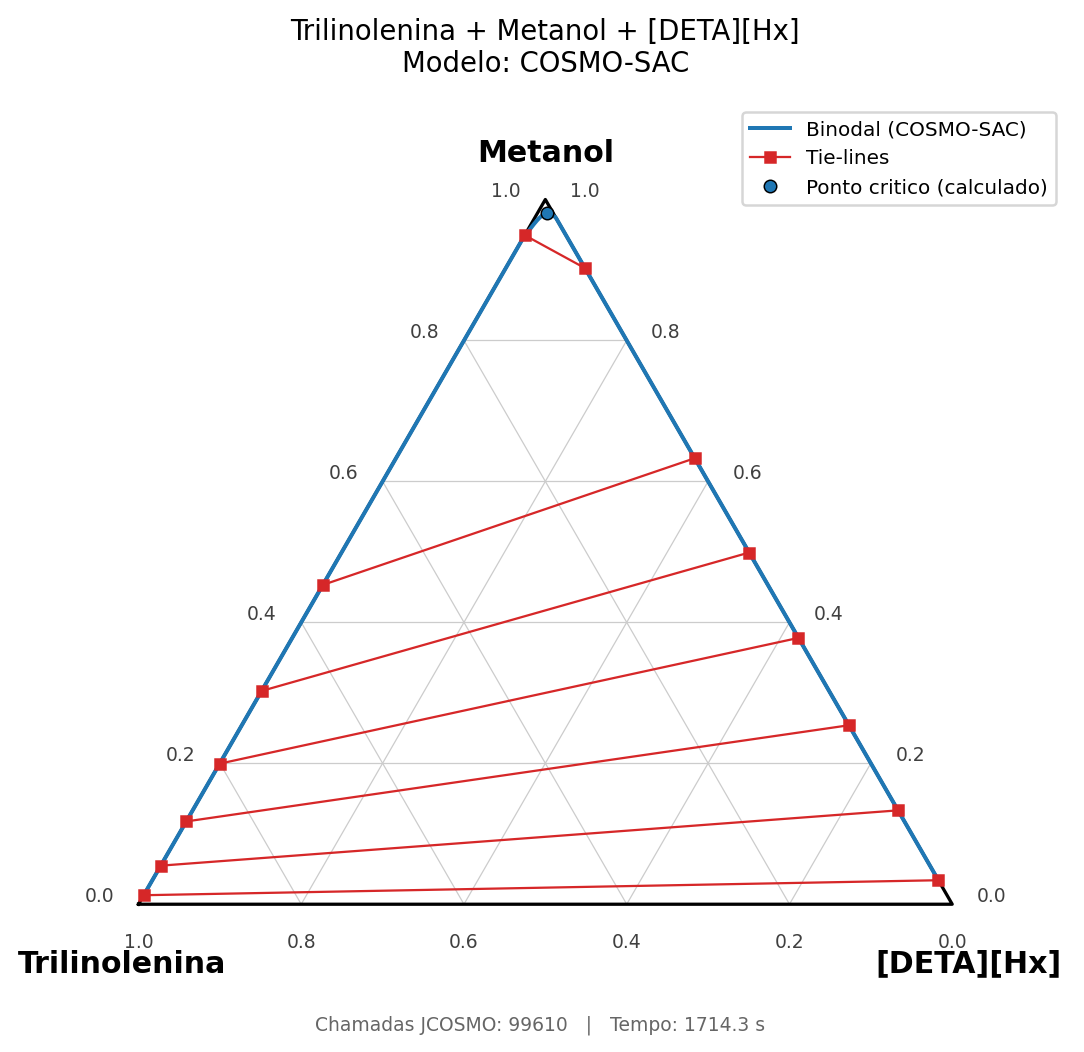
\includegraphics[width=0.4\textwidth]{imagens/ELL_Trilinolenina_Metanol_DETAHx_COSMO_SAC.png}
\caption{Trilinolenina + metanol + [DETA][Hx]: o UNIFAC-LL (esquerda) produz apenas quatro tie-lines confinadas ao vértice do álcool, insuficientes para o traçado da curva; o COSMO-SAC (direita) prevê uma binodal completa}
\label{fig:trilinolenina_metanol_deta}
\end{figure}

A área da região bifásica prevista pelo COSMO-SAC varia entre 0,4659 e 0,4758 nesses seis sistemas (média de 0,4713), portanto acima da média de 0,4214 obtida para os sistemas equivalentes com [2-HEA][Hx] (Seção~\ref{subsec:resultados_2hea}), e à diferença de magnitude soma-se uma diferença de dispersão que merece atenção: enquanto com [2-HEA][Hx] a área percorre uma faixa de aproximadamente 0,07 conforme o triglicerídeo e o álcool empregados (de 0,3819 a 0,4564), com [DETA][Hx] essa faixa se reduz a cerca de 0,01. Sendo assim, na predição do COSMO-SAC, a identidade do triglicerídeo e a do álcool influenciam pouco a extensão da região bifásica quando o [DETA][Hx] está presente, o que sugere que esse líquido iônico prótico domina o comportamento de fases do sistema, ao contrário do que se observa com o [2-HEA][Hx]. O ponto crítico acompanha esse quadro, situando-se consistentemente próximo ao vértice do álcool puro, com fração molar de álcool entre 0,852 e 0,933 e fração de triglicerídeo entre apenas 0,019 e 0,035, o que corresponde a uma região monofásica estável restrita a composições dominadas por álcool quase puro.

A divergência entre os modelos é, nesse conjunto, de natureza categórica, pois eles discordam quanto à própria ocorrência da separação de fases e não apenas quanto ao tamanho da região bifásica. Ela tampouco admite quantificação simétrica, uma vez que do lado do UNIFAC-LL não há região bifásica da qual extrair área ou ponto crítico, o que inviabiliza tanto o cálculo de uma distância entre pontos críticos (como se fez na Seção~\ref{subsec:resultados_2hea}) quanto qualquer forma de valor intermediário entre as duas predições, já que a existência de duas fases líquidas é propriedade qualitativa do sistema e não grandeza que admita interpolação.

Duas observações de plausibilidade cabem ao caso, uma para cada modelo, sem que nenhuma delas resolva a divergência. Do lado do COSMO-SAC, uma região bifásica que ocupa perto de metade do simplex, com ponto crítico tão próximo ao vértice do álcool, implica desestabilização da mistura mesmo em frações muito baixas de triglicerídeo, previsão extrema mas não implausível, visto que cátions poliprotonados são associados na literatura a efeitos de \textit{salting-out} desproporcionais ao seu tamanho molecular, mecanismo retomado na Seção~\ref{subsec:salting_in_out}. Do lado do UNIFAC-LL, a ausência de região bifásica nos seis sistemas depende dos quatro parâmetros de interação preenchidos por completamento de matriz (Seção~\ref{subsec:parametros_perfis}), aplicados aqui a uma combinação (triglicerídeo C57 com cátion amônio triprotonado de cadeia estendida) mais distante da base de treinamento do que a correspondente com [2-HEA][Hx], o que torna a predição menos ancorada, embora não a invalide por si só. Ambas as observações são retomadas na síntese ao final do capítulo (Seção~\ref{subsec:sintese}).

\subsection{Efeito do álcool}
\label{subsec:efeito_alcool}

Mantendo-se fixos o triglicerídeo e o líquido iônico prótico, a substituição do etanol pelo metanol amplia a região de imiscibilidade nos sistemas em que foi possível construir a curva binodal, tendência que já se manifesta no par binário triglicerídeo-álcool, isolado do restante do sistema, uma vez que o coeficiente de atividade em diluição infinita calculado pelo COSMO-SAC para a trioleína em etanol é de 2,61, contra 3,76 em metanol, desvio positivo apreciavelmente mais forte. Esse resultado é coerente com o tamanho da cadeia alquílica de cada álcool, visto que o metanol, por possuir um único átomo de carbono, apresenta superfície molecular proporcionalmente mais dominada pela hidroxila polar do que o etanol, o que reduz sua afinidade com as longas cadeias apolares do triglicerídeo.

A comparação nos diagramas ternários completos abrange nove pares etanol/metanol, correspondentes aos seis pares com [2-HEA][Hx] (três triglicerídeos, em cada um dos dois modelos) somados aos três pares com [DETA][Hx] no COSMO-SAC, ficando de fora os sistemas com [DETA][Hx] no UNIFAC-LL, para os quais não se obteve curva binodal (Seção~\ref{subsec:resultados_deta}) e, por conseguinte, não há área nem ponto crítico a comparar.

Duas medidas apontam no mesmo sentido nesse conjunto. A área da região bifásica é maior com metanol nos nove pares, com aumento entre 1,6\% e 34\% e média em torno de 12\%, ao passo que o ponto crítico desloca-se em direção ao vértice do álcool puro em oito dos nove pares, apresentando fração de álcool superior à do par equivalente com etanol. Considerando-se que essas duas grandezas são obtidas por procedimentos independentes entre si (integração da curva binodal, no primeiro caso, e extrapolação do encolhimento da região instável, no segundo), a convergência entre elas reforça a leitura de que o efeito observado provém do álcool empregado, e dificilmente do método de cálculo.

O número de linhas de amarração acompanha essa tendência nos seis sistemas com [2-HEA][Hx] (Tabela~\ref{tab:tielines_2hea}), nos quais a contagem com metanol supera a com etanol nos dois modelos, mas o mesmo não se verifica nos três sistemas com [DETA][Hx] no COSMO-SAC, em que a contagem cai de 367 para 362 na trioleína e de 370 para 356 na trilinoleína, aumentando apenas na trilinolenina, de 334 para 344 (Tabela~\ref{tab:tielines_deta}). Levando em consideração que a contagem é um indicador da extensão da região bifásica e não uma medida direta dela, conforme observado na abertura desta seção, e que justamente nesses sistemas a área varia numa faixa muito estreita (Seção~\ref{subsec:resultados_deta}), essa discordância pontual não contradiz o que indicam a área e o ponto crítico, embora deva ser registrada em vez de descrever-se a tendência como uniforme.

A diferença entre etanol e metanol aqui caracterizada refere-se ao comportamento de fases a 298,15~K, sem estender-se ao desempenho de cada álcool na reação de transesterificação, no qual entram fatores alheios ao equilíbrio líquido-líquido, como a reatividade do alcóxido correspondente e a estequiometria empregada, de modo que a escolha entre os dois álcoois em processo não decorre diretamente do que se observa nesta seção.

\subsection{Efeito do grau de insaturação}
\label{subsec:insaturacao}

Os três triglicerídeos estudados diferem entre si apenas pelo número de ligações duplas por cadeia graxa, mantendo-se fixo o número de carbonos por cadeia (C18), sendo a trioleína formada por três cadeias monoinsaturadas de ácido oleico, a trilinoleína por três cadeias diinsaturadas de ácido linoleico e a trilinolenina por três cadeias triinsaturadas de ácido linolênico. Cada ligação dupla adicional introduz uma região de maior densidade eletrônica ao longo da cadeia, associada aos elétrons $\pi$ deslocalizados, e reduz a flexibilidade conformacional nesse ponto, pois a geometria planar em torno da ligação dupla impede a livre rotação característica das ligações simples vizinhas, e ambas as alterações modificam discretamente a polarizabilidade da molécula e a distribuição de carga superficial capturada pelo perfil sigma, o que justifica examinar se essa variação estrutural se reflete no comportamento de fases.

A comparação mais controlada disponível é entre trioleína e trilinolenina, os dois triglicerídeos cujos perfis sigma se verificaram geometricamente saudáveis (Seção~\ref{subsec:parametros_perfis}), excluindo-se a trilinoleína pela ressalva do enovelamento. No COSMO-SAC, essa comparação abrange quatro pares, correspondentes às quatro combinações de álcool (etanol e metanol) e líquido iônico prótico ([2-HEA][Hx] e [DETA][Hx]), ao passo que no UNIFAC-LL abrange apenas dois, os pares com [2-HEA][Hx], visto que não se obteve curva binodal para os sistemas com [DETA][Hx] (Seção~\ref{subsec:resultados_deta}), assimetria que convém ter em conta ao ler os resultados adiante.

Nos dois pares disponíveis, o UNIFAC-LL registra aumento da área da região bifásica da trioleína para a trilinolenina, de 66\% no par com etanol e 27\% no par com metanol, enquanto nos quatro pares do COSMO-SAC as áreas resultam praticamente iguais ou ligeiramente menores para a trilinolenina, com variações de $-13\%$, $-9\%$, $-0{,}5\%$ e $-0{,}3\%$. Dois desses quatro valores são de magnitude comparável à incerteza esperada do próprio procedimento de cálculo da área, obtida por integração poligonal sobre as extremidades das linhas de amarração, de modo que o resultado do COSMO-SAC é mais bem descrito como ausência de efeito consistente da insaturação do que como inversão da tendência registrada pelo UNIFAC-LL.

Essa diferença é coerente com a forma como cada modelo representa a insaturação, pois no UNIFAC-LL cada ligação dupla substitui dois grupos \ce{CH2} por um grupo \ce{CH=CH}, alteração discreta na contagem de grupos que se propaga diretamente aos parâmetros $R_k$, $Q_k$ e às interações do grupo C=C, ao passo que no COSMO-SAC a insaturação aparece apenas como uma modulação suave da distribuição de carga superficial da cadeia, sem descontinuidade equivalente. A divergência observada é, portanto, compatível com a estrutura de cada modelo, sem que se possa atribuir maior correção a qualquer das duas representações.

Por conseguinte, a afirmação de que o grau de insaturação altera a miscibilidade dos sistemas estudados precisa vir acompanhada da ressalva de que a direção e a magnitude dessa alteração dependem do modelo empregado, ao contrário do que se observou para o efeito do álcool (Seção~\ref{subsec:efeito_alcool}), no qual as duas medidas independentes apontaram no mesmo sentido nos dois modelos.

A trilinoleína, embora se situe entre as outras duas em número de insaturações, não pode ser incluída nessa comparação com a mesma confiança, pois o enovelamento identificado em seu perfil sigma introduz um viés de superestimação de polaridade que se sobrepõe, e possivelmente mascara, o efeito da insaturação sobre a predição do COSMO-SAC, de modo que não é possível, a partir dos dados deste trabalho, separar quanto da área calculada reflete o grau de insaturação da molécula e quanto reflete a geometria comprometida. Essa ressalva não se aplica ao UNIFAC-LL, que não consome perfil sigma e para o qual a trilinoleína é descrita pela mesma contagem de grupos das demais.

\subsection{Sistemas sem curva binodal obtida}
\label{subsec:casos_sem_separacao}

Nem todos os sistemas avaliados resultaram em curva binodal, e reúnem-se aqui os casos em que isso não ocorreu, junto de um caso que produziu curva mas carrega ressalva relevante. Quando a varredura da grade não identifica composições instáveis, ou identifica um número insuficiente delas para o traçado da curva, registra-se que não foi possível construir a binodal naquelas condições, distinção que não é de forma, uma vez que a ausência de composição instável identificada pelo teste de estabilidade é compatível tanto com uma fase única termodinamicamente estável quanto com uma falha de convergência do procedimento, e os dados deste trabalho não permitem separar as duas hipóteses.

Os dois ácidos graxos livres avaliados, o oleico e o linoleico, correspondentes às cadeias graxas da trioleína e da trilinoleína, não produziram região de instabilidade em nenhuma das combinações testadas com álcool e líquido iônico prótico, de modo que não se obteve curva binodal para nenhum desses sistemas. Registre-se, contudo, que esses resultados provêm de execuções exploratórias, anteriores à consolidação da fila de cálculo empregada nos demais sistemas deste capítulo, e que a exportação formal no mesmo padrão dos demais não foi realizada dentro do escopo deste trabalho, razão pela qual os sistemas com ácido graxo livre figuram aqui como registro de execução, sem o mesmo estatuto dos sistemas com triglicerídeo.

Uma diferença estrutural entre o ácido graxo livre e o triglicerídeo correspondente é, ainda assim, digna de nota, e é retomada na Seção~\ref{subsec:efeito_esterico}. Enquanto as três cadeias esterificadas ao glicerol impõem ao triglicerídeo volume molecular e impedimento estérico consideráveis, o ácido graxo livre expõe um único grupo carboxila terminal (COOH), livre de vizinhança apolar que dispute o mesmo espaço, e portanto disponível para formar ligação de hidrogênio direta com a rede de amônio e carboxilato do líquido iônico. Tal diferença é consistente com a literatura de desacidificação de óleos vegetais que emprega líquidos iônicos de amônio como agente extrator, na qual o mesmo mecanismo é reportado como força motriz da extração, embora se trate de leitura estrutural plausível cuja verificação dependeria dos resultados computacionais que não foram consolidados.

Os dois sistemas de trilinolenina com [DETA][Hx] no UNIFAC-LL (Seção~\ref{subsec:resultados_deta}) apresentam situação diferente, pois a varredura identificou composições instáveis em número reduzido, quatro linhas de amarração com fração de trilinolenina inferior a 0,23 em ambas as fases, confinadas a uma faixa estreita próxima ao vértice do álcool puro. Um conjunto dessa dimensão não permite o traçado de uma curva binodal nem a estimativa do ponto crítico, e a proximidade dessas composições ao limite de estabilidade numérica do algoritmo de flash, combinada à sensibilidade do resultado à malha de composições inicial, desaconselha atribuir significado físico a linhas isoladas nessa região, sem que isso equivalha a afirmar que a região seja necessariamente estável. Implementou-se no código um filtro de número mínimo de linhas de amarração, que identifica automaticamente essa situação e a sinaliza como resultado não conclusivo, de modo que as tabelas deste capítulo já refletem tal depuração.

Já a trilinoleína produziu curva binodal em todos os sistemas avaliados, e a ressalva que a acompanha recai sobre a magnitude do resultado. Conforme discutido na Seção~\ref{subsec:parametros_perfis} e retomado nas Seções~\ref{subsec:resultados_2hea} e~\ref{subsec:insaturacao}, o perfil sigma dessa molécula apresenta conformação enovelada em vez de estendida, o que eleva sua fração polar superficial e tende a superestimar a afinidade calculada com o álcool e com o líquido iônico no COSMO-SAC. Sendo assim, a extensão da região bifásica obtida para a trilinoleína nesse modelo permanece sob ressalva até que a geometria seja reotimizada, ao passo que o resultado do UNIFAC-LL para os mesmos sistemas não é afetado, visto que esse modelo não consome perfil sigma e descreve a trilinoleína pela mesma contagem de grupos funcionais empregada nos demais triglicerídeos.

\section{O líquido iônico prótico atua como cossolvente?}
\label{sec:cossolvencia}

As seções anteriores descreveram o comportamento de fases previsto por cada modelo sem confrontá-lo com a hipótese que motiva o trabalho. A premissa dos estudos experimentais de \citeonline{gomez2019} e \citeonline{trindade2019} é a de que o líquido iônico prótico atua como cossolvente do par triglicerídeo-álcool, isto é, que sua presença aumenta a miscibilidade mútua entre os dois reagentes e, por conseguinte, favorece o contato entre eles no meio reacional. Os diagramas ternários já apresentados permitem examinar essa premissa sem cálculo adicional, uma vez que contêm, no mesmo objeto geométrico, tanto o sistema com cossolvente quanto o sistema sem ele. Definem-se, a seguir, as métricas adotadas para essa leitura e o sistema de referência empregado (Seção~\ref{subsec:metrica_lacuna}); apresentam-se, na sequência, a evolução da lacuna de imiscibilidade (Seção~\ref{subsec:evolucao_lacuna}) e a da solubilidade do triglicerídeo na fase alcoólica (Seção~\ref{subsec:solubilidade_fase_alcoolica}); examina-se, depois, o que a extrapolação para fração nula de líquido iônico indica sobre o par binário (Seção~\ref{subsec:binario_referencia}); e discute-se, por fim, a compatibilidade entre o resultado obtido e os ganhos de rendimento reportados na literatura (Seção~\ref{subsec:regime_concentracao}).

\subsection{Métricas adotadas e sistema de referência}
\label{subsec:metrica_lacuna}

A avaliação do efeito cossolvente exige um ponto de comparação sem cossolvente, e esse ponto está contido no próprio diagrama ternário, pois a aresta que une os vértices do triglicerídeo e do álcool corresponde às composições em que a fração de líquido iônico prótico é nula, de modo que os pontos em que a curva binodal encontra essa aresta descrevem a solubilidade mútua do par binário. Caminhando dali para o interior do triângulo, ao longo de frações crescentes de líquido iônico, obtém-se a resposta do sistema à adição do cossolvente sem necessidade de qualquer cálculo adicional além dos já apresentados na Seção~\ref{sec:resultados_por_sistema}.

Adotam-se duas grandezas para essa leitura. A primeira é a largura da lacuna de imiscibilidade, definida como a diferença de fração molar de triglicerídeo entre os dois ramos da curva binodal (o rico em óleo e o rico em álcool) em um mesmo nível de fração de líquido iônico prótico, e denotada por $\Delta x_{\text{óleo}}$, medida direta da distância entre as duas fases em equilíbrio, já que quanto menor a largura mais próximas em composição estão as fases coexistentes e mais próximo o sistema está da miscibilidade completa. A segunda é a fração molar de triglicerídeo no ramo rico em álcool, isto é, quanto de óleo o meio alcoólico efetivamente comporta, de interesse mais direto para o processo, visto que é essa fase que concentra o álcool disponível para a reação.

O procedimento de cálculo consiste em reunir as composições das extremidades de todas as linhas de amarração de um dado sistema, classificá-las em ramo rico em óleo e ramo rico em álcool, e agrupá-las em dez faixas de fração de líquido iônico prótico, calculando-se em cada faixa a largura média da lacuna e a fração média de óleo na fase alcoólica. Uma vez que os dois extremos de uma mesma linha de amarração não apresentam a mesma fração de líquido iônico (o PIL distribui-se de forma desigual entre as fases, conforme discutido na Seção~\ref{subsec:ligacao_hidrogenio}), adotou-se como fração de referência de cada linha a média entre os valores das duas fases. A tendência de cada sistema é então resumida pela inclinação da regressão linear da largura contra a fração de líquido iônico, $\mathrm{d}(\Delta x_{\text{óleo}})/\mathrm{d}x_{\text{LIP}}$, cujo sinal responde à pergunta desta seção, com inclinação negativa indicando que o líquido iônico aproxima as duas fases, e portanto atua como cossolvente, e inclinação positiva indicando o contrário.

Aplicou-se esse procedimento aos 18 sistemas para os quais se obteve curva binodal, o que abrange os seis sistemas com [2-HEA][Hx] em cada modelo e os seis sistemas com [DETA][Hx] no COSMO-SAC, ficando de fora os sistemas sem curva obtida (Seção~\ref{subsec:casos_sem_separacao}), nos quais não há ramos entre os quais medir distância.

Duas limitações do procedimento devem ser registradas de antemão. A fração de líquido iônico efetivamente amostrada não alcança o zero em nenhum sistema, com a menor faixa disponível situando-se entre 0,047 e 0,316 conforme o caso, de modo que a largura da lacuna na ausência de cossolvente só pode ser estimada por extrapolação das faixas de menor fração. Além disso, todos os cálculos foram conduzidos com a mesma resolução de malha ($n_{\text{grid}} = 20$), sem verificação de convergência em malha mais fina, o que significa que os valores absolutos de largura carregam a incerteza de discretização associada a essa escolha. Sendo assim, a leitura adiante apoia-se preferencialmente no sinal e na ordem de grandeza da inclinação, grandezas que se mostram robustas a esse tipo de incerteza, e trata os valores extrapolados em fração nula de líquido iônico com a cautela correspondente (Seção~\ref{subsec:binario_referencia}).

\subsection{Evolução da lacuna de imiscibilidade com a fração de líquido iônico}
\label{subsec:evolucao_lacuna}

Em todos os 18 sistemas para os quais se obteve curva binodal, sem uma única exceção, a largura da lacuna de imiscibilidade cresce à medida que a fração de líquido iônico prótico aumenta, com inclinações $\mathrm{d}(\Delta x_{\text{óleo}})/\mathrm{d}x_{\text{LIP}}$ entre $+0{,}87$ e $+2{,}95$ (Tabela~\ref{tab:inclinacoes_lacuna}), o que aponta em sentido contrário ao da hipótese de partida. Tampouco se trata de efeito marginal, uma vez que entre a menor e a maior faixa de fração amostrada a largura multiplica-se por um fator que vai de 2,7 a 15,0 conforme o sistema, de modo que a distância entre as composições das duas fases coexistentes chega a ser quinze vezes maior na presença de líquido iônico do que na faixa mais diluída em que foi possível medi-la. Nas condições modeladas neste trabalho, portanto, o líquido iônico prótico não aproxima as fases coexistentes, mas as afasta, comportando-se como agente de separação. Os sistemas com [DETA][Hx] no UNIFAC-LL não constam da tabela, visto que não se obteve curva binodal para eles (Seção~\ref{subsec:resultados_deta}) e, por conseguinte, não há ramos entre os quais medir distância.

\begin{table}[htb]
\centering
\caption{Inclinação da largura da lacuna de imiscibilidade em relação à fração
molar de líquido iônico prótico, nos sistemas com triglicerídeo. As colunas
$\Delta x_{\text{óleo}}$ referem-se à menor e à maior faixa de fração de LIP
amostrada em cada sistema.}
\label{tab:inclinacoes_lacuna}
\begin{tabular}{llccc}
\toprule
Sistema & Modelo & Inclinação
        & $\Delta x_{\text{óleo}}$ (inicial / final) & Razão \\
\midrule
\multicolumn{5}{l}{\textit{Com [2-HEA][Hx]}} \\
Trioleína + Etanol      & COSMO-SAC & $+1{,}71$ & 0,222 / 0,920 & 4,1 \\
Trioleína + Metanol     & COSMO-SAC & $+1{,}36$ & 0,305 / 0,930 & 3,1 \\
Trilinoleína + Etanol   & COSMO-SAC & $+2{,}07$ & 0,217 / 0,916 & 4,2 \\
Trilinoleína + Metanol  & COSMO-SAC & $+1{,}62$ & 0,261 / 0,923 & 3,5 \\
Trilinolenina + Etanol  & COSMO-SAC & $+1{,}82$ & 0,203 / 0,856 & 4,2 \\
Trilinolenina + Metanol & COSMO-SAC & $+1{,}48$ & 0,220 / 0,864 & 3,9 \\
\addlinespace
Trioleína + Etanol      & UNIFAC-LL & $+1{,}25$ & 0,231 / 0,614 & 2,7 \\
Trioleína + Metanol     & UNIFAC-LL & $+0{,}94$ & 0,147 / 0,617 & 4,2 \\
Trilinoleína + Etanol   & UNIFAC-LL & $+1{,}09$ & 0,219 / 0,622 & 2,8 \\
Trilinoleína + Metanol  & UNIFAC-LL & $+0{,}87$ & 0,156 / 0,622 & 4,0 \\
Trilinolenina + Etanol  & UNIFAC-LL & $+0{,}89$ & 0,248 / 0,709 & 2,9 \\
Trilinolenina + Metanol & UNIFAC-LL & $+0{,}88$ & 0,253 / 0,712 & 2,8 \\
\addlinespace
\multicolumn{5}{l}{\textit{Com [DETA][Hx]}} \\
Trioleína + Etanol      & COSMO-SAC & $+2{,}51$ & 0,106 / 0,955 & 9,0 \\
Trioleína + Metanol     & COSMO-SAC & $+1{,}65$ & 0,269 / 0,977 & 3,6 \\
Trilinoleína + Etanol   & COSMO-SAC & $+2{,}95$ & 0,064 / 0,957 & 15,0 \\
Trilinoleína + Metanol  & COSMO-SAC & $+2{,}04$ & 0,149 / 0,978 & 6,6 \\
Trilinolenina + Etanol  & COSMO-SAC & $+2{,}75$ & 0,071 / 0,946 & 13,3 \\
Trilinolenina + Metanol & COSMO-SAC & $+2{,}01$ & 0,158 / 0,972 & 6,2 \\
\bottomrule
\end{tabular}
\end{table}

Essa leitura não depende de arbitrar entre os dois modelos termodinâmicos, já que ambos apontam no mesmo sentido e diferem apenas na intensidade do efeito, com o COSMO-SAC registrando inclinações entre $+1{,}36$ e $+2{,}95$ e o UNIFAC-LL entre $+0{,}87$ e $+1{,}25$, faixas que não chegam a se sobrepor. Levando em consideração que os dois modelos partem de dados de entrada obtidos por vias independentes, parâmetros de interação entre grupos funcionais em um caso e perfis de densidade de carga superficial no outro (Seção~\ref{subsec:parametros_perfis}), a concordância quanto ao sinal da inclinação sugere que o comportamento observado não decorre da parametrização de um deles em particular, ainda que a verificação definitiva dependa de dados experimentais indisponíveis para esses sistemas.

Uma hierarquia entre os dois líquidos iônicos próticos emerge dos resultados do COSMO-SAC, único modelo para o qual há curva nos dois casos, com inclinação média de $+2{,}32$ para o [DETA][Hx] contra $+1{,}67$ para o [2-HEA][Hx], diferença que se mantém quando se comparam os pares equivalentes um a um, como em \{trioleína + etanol\} ($+2{,}51$ contra $+1{,}71$) e em \{trilinoleína + etanol\} ($+2{,}95$ contra $+2{,}07$). O líquido iônico prótico de cátion triprotonado alarga, portanto, a lacuna de forma mais acentuada que o de cátion monoprotonado, resultado coerente com a maior densidade de sítios protonados por unidade de área de superfície discutida adiante (Seção~\ref{subsec:salting_in_out}), pois quanto mais sítios carregados o cátion oferece por área exposta, mais intensa tende a ser sua competição com o triglicerídeo pela hidroxila do álcool.

O efeito do álcool também se manifesta nessa medida, embora de forma que exige alguma atenção para não ser mal interpretada. Em todos os nove pares etanol/metanol comparáveis, a inclinação é maior com etanol do que com metanol, o que à primeira vista parece contradizer a maior imiscibilidade atribuída ao metanol ao longo deste capítulo (Seção~\ref{subsec:efeito_alcool}). A aparente contradição se desfaz ao observar o ponto de partida de cada curva, pois nos sistemas com metanol a largura da lacuna já é substancialmente maior nas menores frações de líquido iônico (0,305 contra 0,222 para a trioleína com [2-HEA][Hx], por exemplo), e essa diferença é ainda mais expressiva do que os números sugerem, uma vez que a medida do metanol foi tomada em $x_{\text{LIP}} = 0{,}047$, contra 0,089 no caso do etanol, isto é, numa condição em que a lacuna deveria ser menor. Caso a lacuna do metanol partisse de um valor comparável ao do etanol, restaria mais espaço para crescimento até o limite geométrico do simplex, e a inclinação seria provavelmente maior. Sendo assim, a inclinação mede a sensibilidade do sistema ao líquido iônico, ao passo que a extensão absoluta da região bifásica permanece maior com metanol, conforme já estabelecido.

\subsection{Solubilidade do triglicerídeo na fase rica em álcool}
\label{subsec:solubilidade_fase_alcoolica}

A largura da lacuna descreve a distância entre as duas fases coexistentes, mas não informa qual delas se desloca, e para o processo interessa em particular a fase rica em álcool, uma vez que é ela que concentra o reagente disponível para a transesterificação, de modo que quanto mais triglicerídeo esse meio comportar, maior o contato entre os reagentes. Examina-se, portanto, a fração molar de triglicerídeo no ramo alcoólico da binodal em função da fração de líquido iônico prótico.

No COSMO-SAC com [2-HEA][Hx], a fase alcoólica torna-se progressivamente mais pobre em triglicerídeo conforme o líquido iônico é adicionado, e a redução alcança ordens de grandeza. Para a trioleína com etanol, a fração de óleo na fase alcoólica cai de $5{,}4 \times 10^{-3}$ na menor faixa de fração de LIP para $2{,}6 \times 10^{-5}$ na maior, redução por um fator de aproximadamente 210, e com metanol o fator é de 188, enquanto nos sistemas com trilinoleína e trilinolenina a mesma tendência se verifica de forma menos acentuada, com fatores entre 20 e 47. Esse comportamento é consistente com o alargamento da lacuna descrito na Seção~\ref{subsec:evolucao_lacuna} e localiza o efeito, pois mostra que o meio alcoólico especificamente perde capacidade de dissolver o triglicerídeo à medida que o líquido iônico prótico se acumula nele.

Nos sistemas com [DETA][Hx], essa mesma leitura esbarra em uma limitação de resolução, já que a fração de triglicerídeo calculada para a fase alcoólica cai abaixo de $10^{-6}$, limiar a partir do qual o algoritmo de flash deste trabalho deixa de distinguir uma composição de zero absoluto (Seção~\ref{subsec:motor_termodinamico}), em oito a dez das dez faixas de cada sistema. Não é possível, por conseguinte, acompanhar a evolução dessa grandeza ao longo da fração de LIP nesses casos, embora se possa registrar que, já nas menores frações amostradas, a fase alcoólica na presença de [DETA][Hx] comporta menos triglicerídeo do que na presença de [2-HEA][Hx] por pelo menos duas ordens de grandeza, o que é coerente com a hierarquia entre os dois líquidos iônicos estabelecida pela métrica anterior.

O UNIFAC-LL não reproduz esse padrão com a mesma nitidez, pois nos seis sistemas com [2-HEA][Hx] a fração de triglicerídeo na fase alcoólica cai em três casos e cresce em três, sempre por fatores entre 1 e 3, sem que a variação alcance uma ordem de grandeza em nenhum deles. A discrepância aparente com a métrica anterior, contudo, se resolve ao examinar separadamente o deslocamento de cada ramo da binodal, uma vez que nesses mesmos seis sistemas o ramo rico em óleo avança entre $+0{,}36$ e $+0{,}47$ em fração molar de triglicerídeo enquanto o ramo alcoólico varia entre $-0{,}024$ e $+0{,}009$, deslocamento de quinze a oitenta vezes menor. O alargamento da lacuna registrado pelo UNIFAC-LL é, portanto, produzido quase inteiramente pelo afastamento do ramo oleoso, e o sinal da variação do ramo alcoólico corresponde a oscilações sobre um movimento de pequena amplitude.

O mesmo mecanismo opera no COSMO-SAC, com magnitude maior, já que nos sistemas equivalentes o ramo oleoso avança entre $+0{,}62$ e $+0{,}69$ enquanto o alcoólico recua entre 0,004 e 0,018. Os dois modelos descrevem, por conseguinte, o mesmo comportamento qualitativo, no qual a adição de líquido iônico prótico enriquece progressivamente a fase oleosa em triglicerídeo sem alterar de forma comparável a composição da fase alcoólica, diferindo apenas quanto ao quanto esse enriquecimento avança. Tal convergência de mecanismo, somada à concordância de sinal já registrada na Seção~\ref{subsec:evolucao_lacuna}, sustenta a leitura de que o líquido iônico prótico atua como agente de separação nas condições modeladas.

\subsection{O comportamento do par binário e o alcance da extrapolação}
\label{subsec:binario_referencia}

A leitura das duas seções anteriores apoia-se em medidas tomadas dentro da faixa de composições efetivamente amostrada, entre frações de líquido iônico prótico de 0,047 e 0,621 conforme o sistema, e resta examinar o que ocorre na direção oposta, ao caminhar em direção à aresta triglicerídeo-álcool, onde a fração de líquido iônico se anula e o sistema se reduz ao par binário. Essa região é a referência natural da análise, mas neste trabalho só pôde ser alcançada por extrapolação.

Extrapolando-se linearmente a largura da lacuna a partir das três faixas de menor fração de líquido iônico de cada sistema, obtêm-se valores negativos em doze dos dezoito casos, entre $-0{,}41$ e $-0{,}02$. Uma largura negativa não tem significado físico, e o que esse resultado indica é que a curva binodal se fecha antes de alcançar a aresta binária, ou seja, que o ponto crítico da região bifásica situa-se em fração de líquido iônico prótico positiva, leitura consistente com a posição do ponto crítico já registrada para os sistemas com [DETA][Hx] no COSMO-SAC (Seção~\ref{subsec:resultados_deta}), na qual a fração de triglicerídeo permanece entre 0,019 e 0,035 e a de álcool entre 0,852 e 0,933.

Os seis sistemas restantes, para os quais a extrapolação fornece largura positiva e portanto lacuna remanescente na aresta binária, são em sua maioria sistemas com metanol (cinco dos seis), de modo que o resultado não é uniforme: a extrapolação sugere binário miscível sobretudo nos sistemas com etanol, enquanto nos sistemas com metanol tende a indicar que a separação de fases persiste mesmo na ausência de líquido iônico prótico. Tal distinção é coerente com a maior imiscibilidade atribuída ao metanol ao longo deste capítulo (Seções~\ref{subsec:efeito_alcool} e~\ref{subsec:evolucao_lacuna}).

Decorre daí uma consequência que se concentra nos sistemas com etanol, pois nas condições modeladas o par binário \{triglicerídeo + etanol\} não apresentaria separação de fases, e a região bifásica só se estabeleceria a partir da adição do líquido iônico prótico. Essa previsão contraria o comportamento experimental conhecido, uma vez que a miscibilidade parcial entre óleo vegetal e álcool de cadeia curta à temperatura ambiente é fato estabelecido e constitui, inclusive, a própria motivação do emprego de cossolventes na transesterificação (Capítulo~\ref{introducao}).

Há um indício independente apontando na mesma direção, e que antecede esta análise. O coeficiente de atividade em diluição infinita calculado pelo COSMO-SAC para a trioleína em etanol é de 2,61 (Seção~\ref{subsec:efeito_alcool}), valor que caracteriza desvio positivo moderado, insuficiente para produzir separação de fases em um sistema binário, para a qual se requerem valores tipicamente uma ordem de grandeza superiores. Esse cálculo refere-se justamente ao par em que a discrepância se manifesta, e o mesmo modelo fornece 3,76 para a trioleína em metanol, valor mais elevado e coerente com a persistência da lacuna extrapolada nesses sistemas. O comportamento do binário obtido por extrapolação da binodal ternária reproduz, portanto, o que o próprio modelo prevê para o binário calculado diretamente, o que afasta a hipótese de erro no procedimento de extrapolação e localiza a discrepância na descrição do par triglicerídeo-álcool pelo modelo.

As inclinações apresentadas na Seção~\ref{subsec:evolucao_lacuna} e os deslocamentos de ramo da Seção~\ref{subsec:solubilidade_fase_alcoolica} foram medidos integralmente dentro da faixa amostrada, sem recurso a extrapolação, e permanecem válidos independentemente do que ocorra na aresta binária, pois o que se estabeleceu é que a lacuna se alarga com a adição de líquido iônico prótico, relação que não pressupõe qualquer valor particular de largura em fração nula. O que a discrepância no binário compromete é a possibilidade de tomar a aresta como referência quantitativa absoluta, isto é, de afirmar quanto da imiscibilidade observada nas frações intermediárias seria atribuível ao líquido iônico e quanto preexistiria no par binário.

Registre-se, por fim, que a extrapolação aqui empregada é linear e apoia-se em três pontos, distantes da origem entre 0,047 e 0,316 em fração de líquido iônico conforme o sistema, o que a torna sensível tanto à escolha do número de faixas quanto à resolução da malha de composições (Seção~\ref{subsec:metrica_lacuna}). Uma verificação com malha mais fina, capaz de amostrar frações de líquido iônico próximas de zero e de determinar diretamente se a binodal alcança ou não a aresta binária, não foi realizada dentro do escopo deste trabalho e constitui a continuação natural desta análise.

\subsection{Compatibilidade com os resultados experimentais de referência}
\label{subsec:regime_concentracao}

Estabelecido que o líquido iônico prótico alarga a lacuna de imiscibilidade nas condições modeladas, resta confrontar esse resultado com as observações experimentais que motivam o trabalho. \citeonline{gomez2019} e \citeonline{trindade2019} reportam ganho de rendimento mássico de biodiesel ao empregar, respectivamente, [2-HEA][Hx] e [DETA][Hx] como cossolventes na transesterificação de óleo de soja, e à primeira vista o alargamento aqui descrito parece contradizer esses ganhos. Três diferenças de escopo, contudo, separam as duas observações a ponto de torná-las compatíveis.

A faixa de concentração é a primeira delas. Os trabalhos de referência empregam o líquido iônico prótico em torno de 2 a 3\% em massa do meio reacional, o que corresponde, para as razões molares álcool/óleo usuais na transesterificação, a frações molares entre aproximadamente 0,005 e 0,028 conforme o líquido iônico considerado, enquanto a menor faixa de fração molar amostrada nos cálculos deste trabalho é de 0,047 (Seção~\ref{subsec:metrica_lacuna}), de modo que o regime experimental situa-se inteiramente abaixo do domínio efetivamente calculado. As inclinações apresentadas na Seção~\ref{subsec:evolucao_lacuna} descrevem, portanto, o comportamento do sistema em concentrações uma a duas ordens de grandeza superiores às empregadas na reação, e sua extensão para a faixa experimental não é assegurada pelos dados aqui obtidos.

A temperatura é a segunda diferença, uma vez que os ganhos de rendimento foram medidos em condição reacional, a aproximadamente 60\,°C, ao passo que os diagramas deste trabalho descrevem o equilíbrio a 298,15~K, condição correspondente à etapa de separação de fases que sucede o resfriamento do meio reacional (Seção~\ref{sec:sistemas}). Trata-se, assim, de duas etapas distintas do mesmo processo, cada uma descrevendo um estado próprio.

A terceira, e mais fundamental, é a natureza da grandeza medida, pois rendimento de reação e equilíbrio líquido-líquido não são a mesma propriedade, e um pode melhorar sem que o outro se altere. Um cossolvente que atue reduzindo a tensão interfacial, ou aumentando a área de contato entre as fases, ou ainda participando da ativação do nucleófilo pelo mecanismo cooperativo descrito no Capítulo~\ref{cap:fundamentacao}, eleva o rendimento sem necessariamente deslocar a curva binodal em direção à miscibilidade completa.

Os resultados da Seção~\ref{subsec:solubilidade_fase_alcoolica} oferecem um argumento adicional nessa direção, já que nos dois modelos a adição de líquido iônico prótico desloca predominantemente o ramo rico em óleo enquanto a composição da fase alcoólica permanece praticamente inalterada. Se o meio alcoólico não passa a comportar mais triglicerídeo, o contato entre reagentes nessa fase tampouco melhora, o que torna a solubilização em fase homogênea uma explicação pouco provável para o ganho de rendimento observado experimentalmente e favorece, por eliminação, os mecanismos de natureza interfacial.

Uma limitação comum aos dois modelos merece registro nesse contexto, pois tanto o UNIFAC-LL quanto o COSMO-SAC descrevem a solução como molecularmente dispersa, na qual cada espécie contribui por sua fração molar e por sua superfície, sem qualquer estrutura de ordem superior, de modo que nenhum deles representa a formação de agregados. Um líquido iônico prótico é, contudo, espécie anfifílica, com porção iônica e cadeia alquílica de seis carbonos no ânion hexanoato (Seção~\ref{subsec:ligacao_hidrogenio}), estrutura compatível com organização em agregados acima de uma concentração crítica, e caso tal organização ocorra nos sistemas reais a solubilização do triglicerídeo no interior desses agregados constituiria um mecanismo de cossolvência que os modelos empregados são, por construção, incapazes de reproduzir. A discrepância entre o comportamento calculado e o experimental pode decorrer, portanto, de uma limitação estrutural compartilhada pelas duas abordagens, hipótese que a modelagem conduzida neste trabalho não permite testar.

A resposta à pergunta que abre esta seção precisa, assim, ser enunciada com o escopo que os dados sustentam. Nas condições modeladas, isto é, a 298,15~K e em frações molares de líquido iônico prótico entre 0,047 e 0,621, a hipótese de cossolvência não se confirma, e os dois modelos indicam que a adição do líquido iônico afasta as fases coexistentes em vez de aproximá-las. Tal resultado não refuta os ganhos de rendimento reportados na literatura, obtidos em temperatura, concentração e grandeza distintas, mas delimita a interpretação desses ganhos, sugerindo que o efeito cossolvente relevante para a transesterificação não se manifesta como aumento de miscibilidade no equilíbrio de fases da etapa de separação.

\section{Interpretação físico-química}
\label{sec:interpretacao_fisicoquimica}

As seções anteriores estabeleceram o que os dois modelos preveem e como a adição de líquido iônico prótico afeta a extensão da região bifásica, sem explicar, em termos de estrutura molecular e de interação intermolecular, por que os sistemas se comportam da forma observada. Tal explicação ganha peso adicional pela ausência de dados experimentais de equilíbrio líquido-líquido para os sistemas específicos deste trabalho (Seção~\ref{sec:dados_validacao}), o que impede a validação direta das predições e desloca parte do valor argumentativo do capítulo para a coerência entre o resultado computacional e o mecanismo que o sustentaria.

Discutem-se aqui três mecanismos que atuam de forma simultânea e não excludente, o impedimento estérico imposto pelas cadeias do triglicerídeo (Seção~\ref{subsec:efeito_esterico}), a competição pelo álcool entre o triglicerídeo e a porção iônica do líquido iônico prótico (Seção~\ref{subsec:salting_in_out}) e a rede de ligações de hidrogênio que ancora o líquido iônico à fase alcoólica (Seção~\ref{subsec:ligacao_hidrogenio}), encerrando-se com uma limitação compartilhada pelas duas abordagens de modelagem, a ausência de representação de agregados (Seção~\ref{subsec:agregacao}).

\subsection{Efeito estérico}
\label{subsec:efeito_esterico}

O primeiro mecanismo é de natureza puramente geométrica. Um triglicerídeo possui três cadeias de ácido graxo esterificadas a um único núcleo de glicerol, o que resulta em molécula volumosa e de baixa razão entre grupos polares (os três grupos éster) e massa apolar (as três cadeias alquílicas longas), configuração que impõe impedimento estérico à aproximação de moléculas de solvente aos sítios polares da molécula, porque qualquer espécie que se aproxime dos grupos éster precisa contornar as cadeias apolares circundantes.

A magnitude desse volume é mensurável diretamente a partir dos cálculos GAMESS realizados para os perfis sigma (Seção~\ref{subsec:parametros_perfis}), pois a cavidade COSMO da trioleína apresenta área de 1143,70~\AA$^2$ e volume de 1277,49~\AA$^3$, contra 399,69~\AA$^2$ e 427,77~\AA$^3$ do ácido oleico livre, que corresponde a uma única das três cadeias que a compõem. O triglicerídeo ocupa, portanto, aproximadamente o triplo do volume da cadeia isolada, mas essa razão esconde o ponto relevante, já que as três cadeias, uma vez ancoradas ao mesmo núcleo, disputam entre si o espaço em torno dos grupos éster, o que reduz a acessibilidade desses grupos ao solvente para além do que a simples soma dos volumes indicaria.

Esse impedimento contribui para explicar a extensão das regiões bifásicas registradas na Seção~\ref{sec:resultados_por_sistema}, que ocupam entre 0,38 e 0,48 do simplex de composições conforme o sistema, pois a baixa miscibilidade do triglicerídeo com a fase alcoólica decorre não apenas da natureza química dos grupos éster, que em princípio poderiam interagir com a hidroxila do álcool, mas também da dificuldade geométrica de expor esses grupos ao meio. Tal leitura é consistente com o comportamento identificado na Seção~\ref{subsec:solubilidade_fase_alcoolica}, na qual o ramo rico em óleo se desloca acentuadamente com a adição de líquido iônico prótico enquanto a fase alcoólica praticamente não incorpora triglicerídeo, o que indica que a barreira à entrada do óleo no meio alcoólico permanece independentemente da quantidade de cossolvente presente.

\subsection{Competição pelo álcool: salting-in e salting-out}
\label{subsec:salting_in_out}

O líquido iônico prótico é espécie anfifílica, com porção polar formada pelo grupo amônio protonado do cátion e pelo grupo carboxilato do ânion, que interage preferencialmente com o álcool, cuja hidroxila oferece sítios compatíveis de doação e aceitação de próton, ao passo que a cadeia alquílica do ânion hexanoato mantém alguma afinidade com a porção apolar do triglicerídeo por meio de interações de dispersão. Essa dupla afinidade caracteriza, em princípio, o comportamento cossolvente clássico, no qual o líquido iônico se posicionaria entre as duas fases, com a porção polar voltada ao álcool e a apolar ao óleo, promovendo a solubilização mútua (efeito de \textit{salting-in}) em vez de intensificar a separação (\textit{salting-out}).

Os resultados da Seção~\ref{sec:cossolvencia} indicam, contudo, que a segunda tendência predomina nas condições modeladas, uma vez que a lacuna de imiscibilidade alarga-se com a adição de líquido iônico prótico em todos os dezoito sistemas avaliados, nos dois modelos, com inclinações entre $+0{,}87$ e $+2{,}95$. Uma leitura física para esse resultado é a competição pelo álcool, pois a porção iônica do líquido iônico prótico estabelece com a hidroxila alcoólica interações mais intensas do que aquelas que o álcool poderia estabelecer com os grupos éster do triglicerídeo, de modo que, à medida que o líquido iônico se acumula na fase alcoólica, reduz-se a disponibilidade de álcool para solvatar o óleo. O cossolvente, nessa leitura, sequestra uma das fases em vez de fazer a ponte entre elas.

A comparação entre os dois líquidos iônicos próticos sustenta essa interpretação. O cátion do [DETA][Hx] é triprotonado, com três grupos amônio distribuídos ao longo de uma cadeia de dietilenotriamina, contra um único grupo amônio no cátion do [2-HEA][Hx], e essa diferença se traduz em densidade de sítios protonados por unidade de área consideravelmente distinta, já que a cavidade COSMO do [2-HEA][Hx] tem área de 235,25~\AA$^2$ e abriga um sítio, o que resulta em 0,00425 sítios/\AA$^2$, enquanto a do [DETA][Hx], com 527,53~\AA$^2$, abriga três sítios, o que resulta em 0,00569 sítios/\AA$^2$, cerca de 34\% mais. Coerentemente, o [DETA][Hx] alarga a lacuna de forma mais acentuada, com inclinação média de $+2{,}32$ contra $+1{,}67$ do [2-HEA][Hx] no COSMO-SAC (Seção~\ref{subsec:evolucao_lacuna}), e exclui o triglicerídeo da fase alcoólica de maneira mais completa, a ponto de a fração de óleo nessa fase cair abaixo do limite de resolução do algoritmo de flash (Seção~\ref{subsec:solubilidade_fase_alcoolica}).

Essa leitura, confrontada com o desempenho experimental relatado na literatura, revela uma tensão aparente. \citeonline{trindade2019} registra, com [DETA][Hx], ganho de rendimento superior ao obtido por \citeonline{gomez2019} com [2-HEA][Hx] em condições comparáveis, o que à primeira vista contradiz a maior capacidade de separação aqui atribuída ao primeiro. A contradição, entretanto, dissolve-se ao considerar que as duas observações se referem a regimes distintos de temperatura e de concentração, conforme discutido na Seção~\ref{subsec:regime_concentracao}, pois o mesmo atributo estrutural, a alta densidade de carga do cátion triprotonado, pode favorecer a ativação cooperativa do nucleófilo na condição reacional (Capítulo~\ref{cap:fundamentacao}) e, simultaneamente, intensificar a competição pelo álcool no equilíbrio de fases a 298,15~K, sem que haja incompatibilidade entre os dois efeitos.

\subsection{Ligação de hidrogênio e distribuição entre as fases}
\label{subsec:ligacao_hidrogenio}

O mecanismo que ancora o líquido iônico prótico à fase alcoólica é a rede de ligações de hidrogênio. O próton lábil ligado ao nitrogênio do cátion amônio, resultante da transferência de próton do ácido hexanoico para a amina durante a síntese (Capítulo~\ref{cap:fundamentacao}), atua simultaneamente como doador e receptor, pois como doador pode ser compartilhado com o oxigênio da hidroxila do álcool ou com o oxigênio do próprio ânion carboxilato do par, e como receptor o par de elétrons livre do nitrogênio permanece disponível para aceitar ligações de outras espécies próticas do meio. Tal capacidade dupla confere ao líquido iônico afinidade particular pela fase alcoólica, na qual a densidade de grupos hidroxila é consideravelmente maior do que na fase rica em triglicerídeo.

Essa afinidade se manifesta na distribuição do líquido iônico prótico entre as fases em equilíbrio, quantificada pelo coeficiente $K_{\text{LIP}} = x_{\text{LIP}}^{\text{álcool}}/x_{\text{LIP}}^{\text{óleo}}$ (Seção~\ref{sec:ell_fundamentos}). Para os sistemas com [2-HEA][Hx], o valor médio situa-se entre 7,3 e 18,4 conforme o triglicerídeo e o álcool (Tabela~\ref{tab:ki_pil}), ou seja, a fase alcoólica retém entre sete e dezoito vezes mais líquido iônico do que a oleosa.

\begin{table}[htb]
\centering
\caption{Coeficiente de distribuição do líquido iônico prótico entre as fases, $K_{\text{LIP}} = x_{\text{LIP}}^{\text{álcool}}/x_{\text{LIP}}^{\text{óleo}}$, calculado pelo COSMO-SAC.}
\label{tab:ki_pil}
\begin{tabular}{lcc}
\toprule
Sistema (com [2-HEA][Hx]) & $K_{\text{LIP}}$ médio & Faixa \\
\midrule
Trioleína + Etanol      & 16,3 & 3,5 -- 21,9 \\
Trioleína + Metanol     & 18,4 & 8,0 -- 22,1 \\
Trilinoleína + Etanol   & 13,0 & 2,3 -- 18,9 \\
Trilinoleína + Metanol  & 14,2 & 3,2 -- 19,1 \\
Trilinolenina + Etanol  & 7,3  & 2,6 -- 9,4  \\
Trilinolenina + Metanol & 7,9  & 3,0 -- 9,5  \\
\bottomrule
\end{tabular}
\end{table}

Para os sistemas com [DETA][Hx], o mesmo coeficiente não pôde ser calculado de forma estatisticamente estável, já que em 77\% a 99\% das linhas de amarração a fração molar de líquido iônico na fase rica em óleo caiu abaixo de $10^{-6}$, limiar a partir do qual o algoritmo de flash deste trabalho deixa de distinguir uma composição de zero absoluto (Seção~\ref{subsec:motor_termodinamico}). Esse valor constitui um limite de resolução do método, e a fração real pode ser ainda menor, mas o padrão sugere exclusão do [DETA][Hx] da fase oleosa mais completa do que a observada para o [2-HEA][Hx], coerente com a densidade de sítios protonados discutida na seção anterior.

A intensidade dessa rede pode ser quantificada a partir dos próprios perfis sigma, integrando-se a área de superfície nas regiões de doação ($\sigma < -0{,}0082$ e/\AA$^2$) e de aceitação ($\sigma > +0{,}0082$ e/\AA$^2$) de ligação de hidrogênio, conforme o critério apresentado na Seção~\ref{sec:cosmo_solvatacao}. Em termos absolutos, o [DETA][Hx] apresenta área ativa quase o dobro da do [2-HEA][Hx] (127,00~\AA$^2$ contra 70,97~\AA$^2$, somadas as duas regiões), o que é consistente com a presença de três ânions hexanoato em vez de um, mas em termos proporcionais a relação se inverte, pois a fração da superfície total dedicada à ligação de hidrogênio é maior no [2-HEA][Hx] (30,1\%) do que no [DETA][Hx] (24,1\%), visto que a cadeia de dietilenotriamina acrescenta área apolar sem acréscimo proporcional de capacidade de ligação.

Essa inversão merece atenção, pois poderia sugerir que o [DETA][Hx], com fração apolar maior (75,9\% contra 69,8\%), toleraria melhor a presença de triglicerídeo, embora os resultados da Seção~\ref{sec:cossolvencia} indiquem o oposto. A explicação plausível é que a competição pelo álcool seja governada pela magnitude absoluta da área ativa somada à densidade de carga do cátion, mais do que pela proporção de superfície dedicada à ligação de hidrogênio, uma vez que uma fração apolar maior oferece, de fato, mais pontos de contato dispersivo com a cadeia do triglicerídeo, porém a interação de dispersão é consideravelmente mais fraca do que a ligação de hidrogênio, e insuficiente para compensar tanto o impedimento estérico da Seção~\ref{subsec:efeito_esterico} quanto o sequestro do álcool descrito na Seção~\ref{subsec:salting_in_out}.

Reunidos os três mecanismos, obtém-se uma descrição coerente do comportamento observado, na qual a rede de ligações de hidrogênio ancora o líquido iônico prótico à fase alcoólica, ele compete ali com o triglicerídeo pela hidroxila do álcool e reduz a capacidade solvente dessa fase, e o impedimento estérico das três cadeias esterificadas impede que a afinidade dispersiva da cauda hexanoato compense essa perda. O resultado líquido é o afastamento progressivo do ramo rico em óleo, com a fase alcoólica praticamente inalterada, que é exatamente o padrão registrado na Seção~\ref{subsec:solubilidade_fase_alcoolica}.

\subsection{Agregação e o limite comum aos dois modelos}
\label{subsec:agregacao}

A descrição construída até aqui apoia-se na premissa de que tanto o UNIFAC-LL quanto o COSMO-SAC tratam a solução como molecularmente dispersa, na qual cada espécie contribui por sua fração molar e por sua superfície, sem qualquer organização de ordem superior, de modo que nenhum dos dois representa a formação de agregados.

Tal premissa é problemática para as espécies em questão, pois o líquido iônico prótico reúne, na mesma molécula, uma porção iônica de alta densidade de carga e uma cadeia alquílica de seis carbonos no ânion hexanoato, arranjo característico de espécies que se organizam em agregados acima de uma concentração crítica, e as frações apolares medidas nos perfis sigma, de 69,8\% para o [2-HEA][Hx] e 75,9\% para o [DETA][Hx] (Seção~\ref{subsec:ligacao_hidrogenio}), indicam que a porção capaz de participar dessa organização é majoritária em área de superfície nos dois casos.

A consequência é direta. Caso agregados se formem nos sistemas reais, o interior apolar dessas estruturas constituiria um ambiente capaz de acomodar cadeias de triglicerídeo dentro da fase alcoólica, o que corresponderia a um mecanismo de cossolvência genuíno, porém invisível para os modelos empregados. Esse mecanismo é compatível com o padrão identificado na Seção~\ref{subsec:solubilidade_fase_alcoolica}, uma vez que um modelo que não representa agregação prevê fase alcoólica incapaz de incorporar óleo, exatamente como se observou, ao passo que o sistema real poderia incorporá-lo por uma via que o modelo desconhece.

Essa limitação é comum às duas abordagens e não distingue uma da outra, pois decorre da hipótese de dispersão molecular que fundamenta ambos os formalismos, em vez de originar-se na parametrização do UNIFAC-LL ou na qualidade dos perfis sigma do COSMO-SAC. A concordância entre os dois modelos quanto ao alargamento da lacuna (Seção~\ref{subsec:evolucao_lacuna}), embora reforce que o resultado não é artefato de uma parametrização específica, tampouco constitui evidência contra a ocorrência de agregação. Verificar essa hipótese exigiria abordagem de outra natureza, como simulação por dinâmica molecular ou determinação experimental da concentração micelar crítica dos dois líquidos iônicos próticos nos meios estudados, e permanece como a limitação mais relevante da modelagem conduzida neste trabalho.

\section{Síntese dos resultados}
\label{subsec:sintese}

Reunidos os resultados apresentados ao longo deste capítulo, distinguem-se três categorias: o que os dois modelos estabelecem em conjunto, aquilo em que divergem e o que permanece indeterminado na ausência de dados experimentais para os sistemas estudados.

O resultado mais firme é o alargamento da lacuna de imiscibilidade com a adição de líquido iônico prótico, verificado nos dezoito sistemas com triglicerídeo para os quais se obteve curva binodal, sem exceção, com inclinações entre $+0{,}87$ e $+2{,}95$ (Seção~\ref{subsec:evolucao_lacuna}). Essa concordância envolve modelos cujos dados de entrada são de naturezas independentes entre si, parâmetros de interação entre grupos funcionais em um caso e perfis de densidade de carga superficial no outro (Seção~\ref{subsec:parametros_perfis}), de modo que o resultado dificilmente se explicaria por uma particularidade da parametrização de qualquer um deles, e o mecanismo subjacente também é comum aos dois, com o alargamento decorrendo quase inteiramente do afastamento do ramo rico em óleo enquanto a composição da fase alcoólica permanece praticamente inalterada (Seção~\ref{subsec:solubilidade_fase_alcoolica}).

Decorre daí a resposta à pergunta que organiza este capítulo. Nas condições modeladas, isto é, a 298,15~K e em frações molares de líquido iônico prótico entre 0,047 e 0,621, a hipótese de cossolvência não se confirma, e o líquido iônico afasta as fases coexistentes em vez de aproximá-las, comportando-se como agente de separação. A interpretação físico-química proposta na Seção~\ref{sec:interpretacao_fisicoquimica} atribui esse comportamento à combinação de três fatores, o ancoramento do líquido iônico à fase alcoólica pela rede de ligações de hidrogênio, a competição resultante pela hidroxila do álcool e o impedimento estérico que impede a cauda hexanoato de compensar essa competição por interação dispersiva com o triglicerídeo.

Dois efeitos secundários apresentam concordância entre os modelos. O metanol produz região bifásica mais extensa que o etanol, o que se verifica na área da binodal em todos os nove pares comparáveis e na posição do ponto crítico em oito deles (Seção~\ref{subsec:efeito_alcool}), enquanto o [DETA][Hx] alarga a lacuna de forma mais acentuada que o [2-HEA][Hx] e exclui o triglicerídeo da fase alcoólica de maneira mais completa, comportamento coerente com a maior densidade de sítios protonados de seu cátion triprotonado (Seção~\ref{subsec:salting_in_out}).

A principal divergência entre os modelos diz respeito à própria ocorrência de separação de fases nos sistemas com [DETA][Hx], nos quais o COSMO-SAC prevê binodal nos seis casos ao passo que no UNIFAC-LL não foi possível construir a curva em nenhum deles (Seção~\ref{subsec:resultados_deta}). A divergência é categórica, não admite quantificação simétrica nem valor intermediário, e os dados deste trabalho não permitem arbitrá-la, restando registrar os elementos disponíveis de cada lado: o perfil sigma do [DETA][Hx] foi verificado quanto à geometria, à estequiometria e à fração polar, sem indício de comprometimento, enquanto os parâmetros de interação empregados pelo UNIFAC-LL para os grupos do líquido iônico provêm de completamento de matriz aplicado a uma combinação molecular ausente da base de treinamento (Seção~\ref{subsec:parametros_perfis}). Esses elementos caracterizam a procedência do dado que produziu cada predição, ainda que a verificação de qualquer uma delas dependa de medida experimental.

Uma segunda divergência, de natureza distinta, aparece no efeito do grau de insaturação, com o UNIFAC-LL associando mais insaturação a região bifásica mais extensa, com aumentos de 27\% e 66\% entre a trioleína e a trilinolenina, ao passo que o COSMO-SAC não registra efeito apreciável, com variações entre $-13\%$ e $-0{,}3\%$ (Seção~\ref{subsec:insaturacao}). Diferentemente do caso anterior, a discordância é aqui de magnitude, e compatível com a forma como cada modelo representa a ligação dupla.

Três limitações delimitam o alcance do conjunto. A impossibilidade de tomar o par binário como referência quantitativa é a primeira, já que a extrapolação da largura da lacuna para fração nula de líquido iônico fornece valores negativos em doze dos dezoito sistemas, o que implicaria par \{triglicerídeo + etanol\} miscível, em desacordo com o comportamento experimental conhecido (Seção~\ref{subsec:binario_referencia}). A distância entre o domínio calculado e o experimental é a segunda, uma vez que as concentrações de líquido iônico empregadas por \citeonline{gomez2019} e \citeonline{trindade2019} correspondem a frações molares uma a duas ordens de grandeza abaixo da menor faixa aqui amostrada (Seção~\ref{subsec:regime_concentracao}). A terceira, e possivelmente a mais restritiva, é a ausência de representação de agregados em ambos os formalismos, que impede avaliar se a cossolvência experimental se realiza por solubilização no interior de estruturas organizadas, mecanismo ao qual os modelos empregados são estruturalmente cegos (Seção~\ref{subsec:agregacao}).

Sendo assim, os resultados deste trabalho descrevem o comportamento de fases dos sistemas \{triglicerídeo + álcool + líquido iônico prótico\} na etapa de separação que sucede o resfriamento do meio reacional, e nessa etapa indicam ação de separação. Tal conclusão não contradiz os ganhos de rendimento reportados na literatura, obtidos em temperatura, concentração e grandeza distintas, mas restringe a interpretação desses ganhos, sugerindo que o efeito cossolvente relevante para a transesterificação não se manifesta como aumento de miscibilidade no equilíbrio líquido-líquido a 298,15~K. Verificar essa leitura exigiria dados experimentais de equilíbrio de fases para os sistemas estudados, inexistentes na literatura até o momento, e a extensão dos cálculos à faixa de baixa concentração de líquido iônico e à temperatura reacional, ambas registradas como continuação natural desta análise.